\documentclass[11pt,a4paper]{article}

%% More layout: Get rid of indenting throughout entire document
\setlength{\parindent}{0in}
            
%Changes from Matthias Althoff:
\usepackage{color,hyperref}
\usepackage{fancyvrb}
\usepackage{eurosym}
%\usepackage[a4paper,left=2.5cm,right=2.5cm,nohead]{geometry}
\usepackage[a4paper,margin=2.5cm]{geometry}
\usepackage{fancyhdr} %for header
\usepackage{titlesec}
\usepackage{enumitem}
\usepackage{tabularx}
\usepackage{lastpage}
\usepackage{parskip}
\usepackage{graphicx}
\usepackage{subfigure}
\usepackage{psfrag}
\usepackage{amsmath,amssymb,amsfonts}
\usepackage{mathrsfs}
\usepackage{cite}
\usepackage{pifont} %for circled numbers
\usepackage{caption}
\usepackage[amsmath,hyperref,thmmarks]{ntheorem}  %better package for proof environment
\usepackage{booktabs}


\newcommand{\mathpzc}[1]{\underline{#1}}
%Indexing elements----------------------
\renewcommand{\^}[1]{^{(#1)}}
\renewcommand{\th}[1]{#1^\text{th}}
%---------------------------------------

\newenvironment{wide_itemize}{
\begin{itemize}
  \setlength{\itemsep}{10pt}
  \setlength{\parskip}{0pt}
  \setlength{\parsep}{0pt}
}{\end{itemize}}

\newenvironment{packed_itemize}{
\begin{itemize}
  \renewcommand{\labelitemi}{$\bullet$}
  \setlength{\itemsep}{2pt}
  \setlength{\parskip}{0pt}
  \setlength{\parsep}{0pt}
}{\end{itemize}}

\newenvironment{first_itemize}{
\setlist{nolistsep}
\vspace{-0.2cm}
\begin{itemize}
  \setlength{\itemsep}{2pt}
  \setlength{\parskip}{0pt}
  \setlength{\parsep}{0pt}
}{\end{itemize}}

\newcommand{\sep}[1]{{\large\textbf{#1}} \vspace{0.3cm}} %seperator

\newcommand{\brake}{\mbox{} \vspace{0cm} \mbox{}} %seperator

%\renewcommand{\sectionmark}[1]{\markright{\thesection\ #1}}



\pagestyle{fancy} %set differnt page style for header
\fancyhead[L]{\leftmark}
\fancyhead[C]{}
\fancyhead[R]{}
\fancyfoot[L]{}
\fancyfoot[C]{\thepage}
\fancyfoot[R]{}


\fancypagestyle{firststyle}
{
   \addtolength{\headheight}{-1.05cm}
   \addtolength{\headsep}{1.05cm}
}


% % easychair.tex,v 3.4 2015/12/10
% 
% \documentclass{easychair}
% %\documentclass[EPiC]{easychair}
% %\documentclass[debug]{easychair}
% %\documentclass[verbose]{easychair}
% %\documentclass[notimes]{easychair}
% %\documentclass[withtimes]{easychair}
% %\documentclass[a4paper]{easychair}
% %\documentclass[letterpaper]{easychair}
% 
% \usepackage{doc}
% 
% % use this if you have a long article and want to create an index
% % \usepackage{makeidx}
% 
% % In order to save space or manage large tables or figures in a
% % landcape-like text, you can use the rotating and pdflscape
% % packages. Uncomment the desired from the below.
% %
% % \usepackage{rotating}
% % \usepackage{pdflscape}
% 
% % Some of our commands for this guide.
% %
% \newcommand{\easychair}{\textsf{easychair}}
% \newcommand{\miktex}{MiK{\TeX}}
% \newcommand{\texniccenter}{{\TeX}nicCenter}
% \newcommand{\makefile}{\texttt{Makefile}}
% \newcommand{\latexeditor}{LEd}
% 
% %Changes from Matthias Althoff:
% \usepackage{color,hyperref}
% \usepackage{fancyvrb}
% \usepackage{eurosym}
% \usepackage{titlesec}
% \usepackage{enumitem}
% \usepackage{tabularx}
% \usepackage{lastpage}
% \usepackage{parskip}
% \usepackage{graphicx}
% \usepackage{subfigure}
% \usepackage{psfrag}
% \usepackage{amsmath,amssymb,amsfonts}
% \usepackage{mathrsfs}
% \usepackage{cite}
% \usepackage{pifont} %for circled numbers
% \usepackage{caption}
% \usepackage{booktabs}
% %\usepackage{breakurl}

% \newtheorem{lemma}{Lemma}
% \newtheorem{definition}{Definition}[]
% \newtheorem{proposition}{Proposition}[]

\DeclareMathOperator{\arccosh}{arccosh}
\DeclareMathOperator{\arcsinh}{arcsinh}
\DeclareMathOperator{\arctanh}{arctanh}
\DeclareMathOperator{\abs}{abs}
\DeclareMathOperator{\sign}{sgn}

\newcommand{\cmark}{\ding{51}}%
\newcommand{\xmark}{\ding{55}}
\renewcommand{\a}{l_f} %vehicle parameter
\renewcommand{\b}{l_r} %vehicle parameter
\newcommand{\prho}{\rho} %vehicle parameter
\newcommand{\pA}{A} %vehicle parameter
\newcommand{\sX}{\sum X} %auxiliary vehicle variable
\newcommand{\sN}{\sum N} %auxiliary vehicle variable
\newcommand{\sY}{\sum Y} %auxiliary vehicle variable
\newcommand{\sL}{\sum L} %auxiliary vehicle variable
\newcommand{\sZ}{\sum Z} %auxiliary vehicle variable
\newcommand{\sM}{\sum M} %auxiliary vehicle variable


\begin{document}

\mbox{} \vspace{0.8cm} \mbox{}
\begin{center} {\Huge\textbf{CommonRoad: Vehicle Models} \\[0.3cm] \huge(Version 2019b)} \end{center}
\vspace{0.2cm}
\begin{center} {\large Matthias Althoff} \\[0.2cm] Technische Universit\"at M\"unchen, 85748 Garching, Germany
\end{center}
\vspace{0.2cm}

\noindent

\begin{abstract}
This document presents models in \textit{CommonRoad} for vehicle dynamics ranging from simple to complicated: The simplest model is a point-mass model, while the most complicated one is a multi-body model. All models are presented in state-space form to facilitate their implementation in standard solvers for ordinary differential equations. We further provide parameter sets and a precise initialization of the multi-body model. To be able to compare the results with simpler models, it is presented how the initial states and the parameters of the multi-body model can be transfered to simpler models. Implementation examples in MATLAB and Python are provided on the \textit{CommonRoad} website. Our repository also provide routines to convert initial states and parameters. Simulation examples demonstrate the advantages of more complicated models.
\end{abstract}


\setcounter{tocdepth}{2}
{\small
\tableofcontents}


%\pagestyle{empty}

%------------------------------------------------------------------------------
\section{Introduction}
\label{sec:introduction}

This document is part of the \textit{CommonRoad} benchmark repository for motion planning of road vehicles, alongside other documents for possible cost functions and road scenarios. It is assumed in this document that all vehicles have an underlying controller that can realize a commanded acceleration (positive and negative). Especially for adaptive cruise control, numerous works already exist that realize a commanded acceleration, see e.g. \cite{Shladover1991,Kim2007}. The effects on engine characteristics in terms of fuel consumption can be considered in the cost function as demonstrated in the document on cost functions.

The lateral dynamics, however, cannot be abstracted away to the same extent using controllers. Especially, when constraints such as the danger of roll-over have to be considered in extreme maneuvers \cite{Odenthal1999, Gaspar2005}. For this reason, our models consider increasingly complicated lateral vehicle dynamics and tire models: point-mass model, kinematic single-track model, single-track model, and a multi-body model. For each model, we (1) present the set of required ordinary differential equations, (2) convert them into state-space form so that common solvers can be used, and (3) provide typical parameters.

In \textit{CommonRoad}, we provide three types of vehicles: 
\begin{itemize}
 \item a small vehicle (Ford Escort; vehicle ID: 1), 
 \item a medium vehicle (BMW 320i; vehicle ID: 2), 
 \item and a van (VW Vanagon; vehicle ID: 3).
\end{itemize}
Detailed parameters of these vehicles have been collected from \cite[Appendix A]{Allen1992} and other vehicle databases that are online available. For each vehicle, we provide the aforementioned models: point-mass model (Sec.~\ref{sec:PMmodel}), kinematic single-track model (Sec.~\ref{sec:KSmodel}), single-track model (Sec.~\ref{sec:STmodel}), and a multi-body model (Sec.~\ref{sec:MBmodel}). After combining the vehicle identifier with the model type, one obtains the model ID. For instance, KS2 is a kinematic single-track model using the parameters of the BMW 320i. In addition, we describe in Sec.~\ref{sec:conversion} how parameters and initial states can be converted from complicated to simpler models. Finally, in Sec.~\ref{sec:examples} we provide some numerical results.

\section{Changes Compared to Version 2019a}

The vehicle models did not change compared to version 2019a. Only the presentation for the kinematic single-track model has changed: it is now clarified that the reference point is the center of the rear axle and not the center of mass.

\section{Steering and Acceleration Constraints} \label{sec:constraints}

With the exception of the point-mass model, all vehicle models respect steering and acceleration constraints. Since the point mass model only uses acceleration as an input, no steering constraints can be modeled. To formulate the constraints, let us first introduce the steering angle $\delta$, the velocity of the steering angle $v_\delta$, the velocity $v$, and the parameter $v_S$ describing the velocity above which the engine power is not sufficient to cause wheel slip. We denote by $\underline{\square}$ the minimum possible value and by $\overline{\square}$ the maximum possible value and by $\square_\mathtt{lat}$ the value of a variable in lateral direction and by $\square_\mathtt{long}$ the value in longitudinal direction. 

The constraints on steering angle velocity, steering angle, and velocity are straightforward:
\begin{equation}
 v_\delta \in [\underline{v}_\delta, \overline{v}_\delta], \quad \delta \in [\underline{\delta}, \overline{\delta}], \quad v \in [\underline{v}, \overline{v}]. \label{eq:remainingRestrictions}
\end{equation}
Considering limited engine power and braking power results in the following constraint as detailed in \cite[Sec.~III.B]{Althoff2016d}:
\begin{equation}
 a_\mathtt{long} \in [\underline{a},\overline{a}(v)], \quad \overline{a}(v) = \begin{cases}
                                                                                            a_\mathtt{max}\frac{v_S}{v} & \text{for } v > v_S, \\
                                                                                            a_\mathtt{max} & \text{otherwise}.
                                                                                           \end{cases} \label{eq:longitudinalRestriction} 
\end{equation}
Finally, we consider the friction circle (aka Kamm's circle) limiting absolute acceleration:
\begin{equation}
\sqrt{a_\mathtt{long}^2 + (v\, \dot{\Psi})^2} \leq a_\mathtt{max} \qquad (a_\mathtt{lat} = v\, \dot{\Psi}) \label{eq:lateralRestriction} 
\end{equation}
The constraints on steering, velocity, and acceleration can be directly considered by introducing a desired steering velocity $v_{\delta,d}$ and a desired acceleration $a_\mathtt{long,d}$ as well as choosing 
\begin{flalign} 
 v_{\delta} = f_{steer}(\delta,v_{\delta,d}) = & \begin{cases}
                0 & \text{ for } (\delta \leq \underline{\delta} \land v_{\delta,d} \leq 0) \lor (\delta \geq \overline{\delta} \land v_{\delta,d} \geq 0) \quad (C1), \\
                \underline{v}_\delta & \text{ for } \lnot C1 \land v_{\delta,d} \leq \underline{v}_\delta, \\
                \overline{v}_\delta & \text{ for } \lnot C1 \land v_{\delta,d} \geq \overline{v}_\delta, \\
                v_{\delta,d} & \text{ otherwise},
               \end{cases} \label{eq:steeringRestriction} \\
 a_\mathtt{long} = f_{acc}(v, a_\mathtt{long,d}) = & \begin{cases}
                0 & \text{ for } (v \leq \underline{v} \land a_\mathtt{long,d} \leq 0) \lor (v \geq \overline{v} \land a_\mathtt{long,d} \geq 0) \quad (C2), \\
                \underline{a} & \text{ for } \lnot C2 \land a_\mathtt{long,d} \leq \underline{a}, \\
                \overline{a}(v) & \text{ for } \lnot C2 \land a_\mathtt{long,d} \geq \overline{a}(v), \\
                a_\mathtt{long,d} & \text{ otherwise}.
               \end{cases} \label{eq:accelerationRestriction}
\end{flalign}
Constraint parameters for different vehicle models are listed in Tab.~\ref{tab:constraintParameters}.

\begin{table}[h]
\caption{Constraint Parameters (obtained from information on the Internet). }
{\small
\begin{center}\label{tab:constraintParameters}
\begin{tabular}{lllclll}
	\toprule
	\multicolumn{3}{c}{\textbf{vehicle parameter}} & \phantom{a} & \multicolumn{3}{c}{\textbf{vehicle identifier}} \\ \cmidrule{1-3} \cmidrule{5-7} 
	\textbf{name} & \textbf{symbol} & \textbf{unit} && \textbf{1} & \textbf{2} & \textbf{3}  \\ \hline
	minimum steering angle & $\underline{\delta}$ & [rad] && $-0.910$ & $-1.066$ & $-1.023$ \\ 
	maximum steering angle & $\overline{\delta}$ & [rad] && $0.910$ & $1.066$ & $1.023$ \\ 
	minimum steering velocity & $\underline{v}_\delta$ & [rad/s] && $-0.4$ & $-0.4$ & $-0.4$ \\ 
	maximum steering velocity & $\overline{v}_\delta$ & [rad/s] && $0.4$ & $0.4$ & $0.4$ \\ 
	min. velocity (also depending on traffic rules) & $\underline{v}$ & [m/s] && $-13.9$ & $-13.6$ & $-11.2$ \\ 
	max. velocity (also depending on traffic rules) & $\overline{v}$ & [m/s] && $45.8$ & $50.8$ & $41.7$ \\ 
	switching velocity & $v_S$ & [m/s] && $4.755$ & $7.319$ & $4.824$ \\ 
	maximum acceleration & $a_\mathtt{max}$ & [m/s$^2$] && $11.5$ & $11.5$ & $11.5$ \\
	\bottomrule 
\end{tabular}
\end{center}}
\end{table}

% 1989 Ford Escort: power: 67kW, top speed: 165 km/h, turning radius: 10.88m, length: 4.298m, width: 1.674m; reverseGearRatio: 3.27; velMax*gearRatio [m/s]: 45.4750; max. backwad velocity: 13.9067
% 1981 BMW 320i: Power: 92kW, top speed: 183 km/h, turning radius: 10.3m, length: 4.508m (with US bumpers), width: 1.610m; reverseGearRatio: 3.682; velMax*gearRatio [m/s]: 50.1161; max. backwad velocity: 13.9067
% 1984 VW Vanagon: Power: 82kW, top speed: 150 km/h, turning radius: 10.7m, length: 4.569m, width: 1.844m; reverseGearRatio: 3.67; velMax*gearRatio [m/s]: 40.9887; max. backwad velocity: 11.1686
% delta_max = arctan(l/R); only for bicycle model
% delta_max = arcsin(2*l/R); according to German Wiki entry
% v_s = P_max/(m*a_max)

We would also like to mention, that other works do not provide all the constraints presented in this document (which can be easily removed, but a removal should be stated since this simplifies motion planning). 

\section{Point-Mass Model (PM)} \label{sec:PMmodel}

The point-mass model is the simplest model that is commonly used for motion planning, see e.g. \cite{Tomas-Gabarron2013,Godbole1997}. This model abstracts the vehicle as a point mass that can be accelerated within bounds. This bound is typically chosen as a circle (Kamm's circle), which is also the bound chosen in this benchmark suite. Let us introduce $\square$ as the placeholder for a variable and $\square_x$ and $\square_y$ to denote the value of the corresponding variable in $x$ and $y$ direction, respectively. After further introducing position $s$, acceleration $a$, and maximum absolute acceleration $a_\mathtt{max}$, the dynamics of the point mass model is
\begin{flalign*}
 \ddot{s}_x = a_x, \quad \ddot{s}_y = a_y, \quad \sqrt{a_x^2 + a_y^2} \leq a_\mathtt{max}. &&
\end{flalign*}
The point-mass model ignores that vehicles have a minimum turning circle, which is considered in the kinematic single-track model. 

\subsection{State Space Model}

After introducing the state variables $x_i$ as 
\begin{flalign*}
  x_1 = s_x, \quad x_2 = s_y, \quad x_3 = \dot{s}_x, \quad x_4 = \dot{s}_y &&
\end{flalign*}
and the input variables $u_i$ as
\begin{flalign*}
  u_1 = a_x, \quad u_2 = a_y, && 
\end{flalign*}
the system dynamics can be written as the linear system
\begin{flalign*}
 \dot{x} = Ax + Bu, \qquad A=\begin{bmatrix} 0 & 0 & 1 & 0 \\ 0 & 0 & 0 & 1 \\ 0 & 0 & 0 & 0 \\ 0 & 0 & 0 & 0 \end{bmatrix}, \quad B = \begin{bmatrix} 0 & 0 \\ 0 & 0 \\ 1 & 0 \\ 0 & 1 \end{bmatrix}. &&
\end{flalign*}
The only constraint in state space form is $\sqrt{u_1^2 + u_2^2} \leq a_\mathtt{max}$. 

\subsection{Parameters}

The only parameter of this model is $a_\mathtt{max}$. Since in this version all vehicles use the same tire, we have $a_\mathtt{max} = 11.5$ [m/s$^2$] (see Tab.~\ref{tab:constraintParameters}).

\section{Kinematic Single-Track Model (KS)} \label{sec:KSmodel}

The kinematic single-track models a road vehicle with only two wheels, where the front and rear wheel pairs are each lumped into one wheel. This simplification is justified since the roll dynamics is not considered (see Fig.~\ref{fig:bicycleModel} and \cite[Sec.~2.2]{Rajamani2012}). This also explains the term \textit{single-track model}. The kinematic single-track model further does not consider any tire slip, so that the velocity vector $v$ at the center of the rear axle is always aligned with the link between the front and rear wheel as depicted in Fig.~\ref{fig:kinematicBicycleModel}. Similarly to the point-mass model, the kinematic single-track model is used in many works for motion planning, e.g. \cite{Paden2016,Petti2005}. A simple example, where the benefit of a kinematic single-track model is evident, is parking: a point-mass model is not sufficient since it would not consider the non-holonomic behavior and in particular the minimum turning radius. 

In addition to the variables already introduced for the point-mass model and the already introduced velocity $v$, we additionally require the velocity of the steering angle $v_\delta$, the steering angle $\delta$, the heading $\Psi$, and the parameter $l_{wb}$ describing the wheelbase. The differential equations of the kinematic single-track model as defined in this document are
\begin{flalign} \label{eq:KS}
 \dot{\delta} = & v_\delta, && \nonumber \\
 \dot{\Psi} =  & \frac{v}{l_{wb}} \tan(\delta), \nonumber \\
 \dot{v} =     & a_\mathtt{long}, \\
 \dot{s}_x =   & v \cos(\Psi), \nonumber \\
 \dot{s}_y =   & v \sin(\Psi), \nonumber 
\end{flalign}
Please note that kinematic single-track models slightly differ in publications, depending on whether one considers that (1) the steering angle or the steering velocity is an input or (2) the vehicle velocity or the vehicle acceleration is an input. For instance, in \cite[eq.~(8)]{Paden2016}, the vehicle velocity and the steering velocity are inputs. 

\begin{figure}[h]
    \centering		
    \footnotesize		
      \psfrag{a}[c]{$\begin{bmatrix} s_x \\ s_y \end{bmatrix}$}									 
      \psfrag{b}[c]{$\Psi$}	    	  
      \psfrag{d}[c]{$l_{wb}$}
      \psfrag{f}[c]{$\delta$}
      \psfrag{x}[c]{$x$}
      \psfrag{y}[c]{$y$}
      \psfrag{v}[c]{$v$}						 
			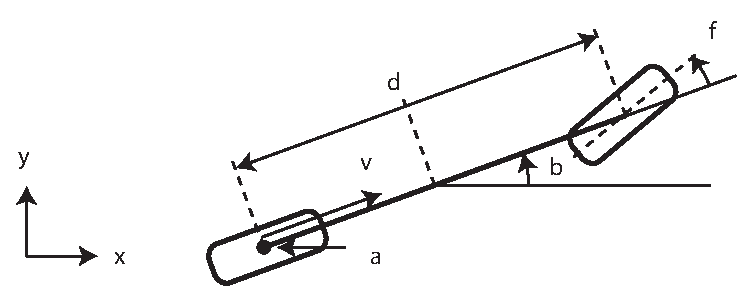
\includegraphics[width=10cm]{./figures/kinematicBicycleModel.eps}
      \caption{Kinematic single-track model.}
      \label{fig:kinematicBicycleModel}
\end{figure}

\subsection{State Space Model}

To write the kinematic single-track model in state-space form, we introduce the following state variables:
\begin{flalign*}
  x_1 = s_x, \quad x_2 = s_y, \quad x_3 = \delta, \quad x_4 = v, \quad  x_5 = \Psi. &&
\end{flalign*}
The input variables are
\begin{flalign} \label{eq:inputVariables}
  u_1 = v_\delta, \quad u_2 = a_\mathtt{long}. &&
\end{flalign}
Inserting the state and input variables into \eqref{eq:KS} and directly considering the constraints on steering, velocity, and acceleration, results in
\begin{flalign*} 
 \dot{x}_1 = & x_4 \cos(x_5), \\
 \dot{x}_2 = & x_4 \sin(x_5), \\
 \dot{x}_3 = & f_{steer}(x_3, u_1), && \text{see \eqref{eq:steeringRestriction}} \\
 \dot{x}_4 = & f_{acc}(x_4, u_2), && \text{see \eqref{eq:accelerationRestriction}} \\
 \dot{x}_5 = & \frac{x_4}{l_{wb}} \tan(x_3).
\end{flalign*}
Because the constraints on steering, velocity, and acceleration are already considered by $f_{steer}(x_3, u_1)$ and $f_{acc}(x_4, u_2)$, it only remins to consider the friction circle:
\begin{equation} \label{eq:KSconstraints}
\begin{split}
 & \sqrt{u_2^2 + (x_4\, \dot{x}_5)^2} \leq a_\mathtt{max}.
\end{split}
\end{equation}

\subsection{Parameters}

The parameters of this model are listed in Tab.~\ref{tab:vehicleParametersKS} and the constraint parameters are presented in Tab.~\ref{tab:constraintParameters}.


\begin{table}[h]
\caption{Vehicle Parameters for the kinematic single-track model (values have been obtained according to Sec.~\ref{sec:parameterConversion}). }
{\small
\begin{center}\label{tab:vehicleParametersKS}
\begin{tabular}{lllclll}
	\toprule
	\multicolumn{3}{c}{\textbf{vehicle parameter}} & \phantom{a} & \multicolumn{3}{c}{\textbf{vehicle identifier}} \\ \cmidrule{1-3} \cmidrule{5-7} 
	\textbf{name} & \textbf{symbol} & \textbf{unit} && \textbf{1} & \textbf{2} & \textbf{3}  \\ \hline
	vehicle length & $l$ & [m] && $4.298$ & $4.508$ & $4.569$ \\
	vehicle width & $w$ & [m] && $1.674$ & $1.610$ & $1.844$ \\
	wheelbase & $l_{wb}$ & [m] && $2.391$ & $2.578$ & $2.471$ \\ 
	\bottomrule %LR
\end{tabular}
\end{center}}
\end{table}





\section{Single-Track Model (ST)} \label{sec:STmodel} 

Since the kinematic single-track model does not consider tire slip, important effects such as understeer or oversteer are not considered \cite[Sec.~2.3]{Rajamani2012}. However, when the vehicle is not driving close to its physical capabilities, those effects are not dominant. The extension is the well-known single-track model, which is also known as the bicycle model. Works that perform planning of evasive maneuvers closer to physical limits require the single-track model, see e.g. \cite{Jeon2011,Shiller1991}. We additionally consider the load transfer of the vehicle due to longitudinal acceleration $a_\mathtt{long}$ (neglecting suspension dynamics), such that the vertical forces on the front and rear axis $F_{z,f}$ and $F_{z,r}$ become
\begin{flalign*}
 F_{z,f} = \frac{mg l_r - m a_\mathtt{long} h_{cg}}{l_r+l_f}, \quad 
 F_{z,r} = \frac{mg l_f + m a_\mathtt{long} h_{cg}}{l_r+l_f}, &&
\end{flalign*}
with parameters from Tab. \ref{tab:vehicleParametersST}. These forces are inserted into the derivation of the equations for the slip angle (at the center of gravity) $\beta$ and the yaw rate $\dot{\Psi}$ \cite[Sec.~2.3]{Rajamani2012}. Using the previously introduced variables and the parameters in Tab. \ref{tab:vehicleParametersST}, the single-track model as defined in this work is
\begin{flalign} \label{eq:ST}
 \dot{\delta} = & v_\delta, \nonumber \\
 \dot{\beta} = & \frac{\mu}{v(l_r + l_f)} \Big( C_{S,f}(g l_r - a_\mathtt{long} h_{cg}) \delta 
                 - (C_{S,r}(g l_f + a_\mathtt{long} h_{cg}) + C_{S,f}(g l_r - a_\mathtt{long} h_{cg})) \beta && \nonumber \\
               & + (C_{S,r}(g l_f + a_\mathtt{long} h_{cg})l_r - C_{S,f}(g l_r - a_\mathtt{long} h_{cg})l_f) \frac{\dot{\Psi}}{v} \Big) - \dot{\Psi}, \nonumber \\
 \ddot{\Psi} = & \frac{\mu m}{I_z(l_r + l_f)} \Big( l_f C_{S,f} (g l_r - a_\mathtt{long} h_{cg}) \delta \\
               & + \left( l_r C_{S,r}(g l_f + a_\mathtt{long} h_{cg}) - l_f C_{S,f} (g l_r - a_\mathtt{long} h_{cg}) \right) \beta \nonumber \\
               & - \left(l_f^2 C_{S,f} (g l_r - a_\mathtt{long} h_{cg}) + l_r^2 C_{S,r}(g l_f + a_\mathtt{long} h_{cg}) \right) \frac{\dot{\Psi}}{v} \Big), \nonumber \\
 \dot{v} =     & a_\mathtt{long}, \nonumber \\
 \dot{s}_x =   & v \cos(\beta + \Psi), \nonumber \\
 \dot{s}_y =   & v \sin(\beta + \Psi), \nonumber
\end{flalign}
under consideration of \eqref{eq:remainingRestrictions}-\eqref{eq:lateralRestriction}. Please note that in contrast to this work, other works often only consider constant velocity when referring to a single-track model (see e.g. \cite[Sec.~2.3]{Rajamani2012}). Also, the weight transfer between the front and rear axle is often neglected in single-track models (see e.g. \cite{Jeon2011}). Note that we do not use the cornering stiffness $C$, as is typically done for single-track models, but separate the effect of the friction coefficient $\mu$, the cornering stiffness coefficient $C_{S}$, and the vertical force $F_z$, such that $C_i = \mu C_{S,i} F_{z,i}$ and $i=\{f,r\}$ for the front and rear axle. This separation is done because the friction coefficient is the most dominant parameter modeling the influence of weather. 

\begin{figure}[h]
    \centering		
    \footnotesize		
      \psfrag{a}[c]{$\begin{bmatrix} s_x \\ s_y \end{bmatrix}$}									 
      \psfrag{b}[c]{$\Psi$}	    
      \psfrag{c}[c]{$\beta$}	  
      \psfrag{d}[c]{$l_r$}
      \psfrag{e}[c]{$l_f$}
      \psfrag{f}[c]{$\delta$}
      \psfrag{x}[c]{$x$}
      \psfrag{y}[c]{$y$}
      \psfrag{v}[c]{$v$}						 
			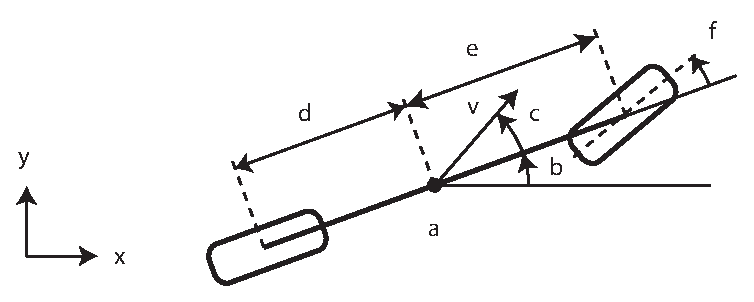
\includegraphics[width=10cm]{./figures/bicycleModel.eps}
      \caption{Single-track model.}
      \label{fig:bicycleModel}
\end{figure}



\subsection{State Space Model}

The single-track model requires a few more state variables compared to the kinematic single-track model. In order to share the constraint function in \eqref{eq:KSconstraints}, we keep the numbering of state variables shared with the kinematic single-track model:
\begin{flalign*}
  x_1 = s_x, \quad x_2 = s_y, \quad x_3 = \delta, \quad x_4 = v, \quad x_5 = \Psi, \quad x_6 = \dot{\Psi}, \quad x_7 = \beta. &&
\end{flalign*}
The input variables are identical to \eqref{eq:inputVariables}. Inserting the state and input variables into \eqref{eq:ST} and directly considering the constraints on steering, velocity, and acceleration, results in the single-track model for $\mathbf{|x_4|\geq0.1}$:
\begin{flalign} 
 \dot{x}_1 = & x_4 \cos(x_5 + x_7), && \nonumber \\
 \dot{x}_2 = & x_4 \sin(x_5 + x_7), \nonumber \\
 \dot{x}_3 = & f_{steer}(x_3, u_1), && \text{see \eqref{eq:steeringRestriction}} \nonumber \\
 \dot{x}_4 = & f_{acc}(x_4, u_2), && \text{see \eqref{eq:accelerationRestriction}} \nonumber \\
 \dot{x}_5 = & x_6, \nonumber \\
 \dot{x}_6 = & \frac{\mu m}{I_z(l_r + l_f)} \Big(l_f C_{S,f} (g l_r - u_2 h_{cg}) x_3 + \left( l_r C_{S,r}(g l_f + u_2 h_{cg}) - l_f C_{S,f} (g l_r - u_2 h_{cg}) \right) x_7 \nonumber \\
               & - \left(l_f^2 C_{S,f} (g l_r - u_2 h_{cg}) + l_r^2 C_{S,r}(g l_f + u_2 h_{cg}) \right) \frac{x_6}{x_4} \Big), \nonumber \\
 \dot{x}_7 = & \frac{\mu}{x_4(l_r + l_f)} \Big( C_{S,f}(g l_r - u_2 h_{cg}) x_3 - (C_{S,r}(g l_f + u_2 h_{cg}) + C_{S,f}(g l_r - u_2 h_{cg})) x_7 \nonumber \\
               & + (C_{S,r}(g l_f + u_2 h_{cg})l_r - C_{S,f}(g l_r - u_2 h_{cg})l_f) \frac{x_6}{x_4} \Big) - x_6. \label{eq:slipAngle_ST}
\end{flalign}
Due to the special choice of state variables, the constraint is identical to \eqref{eq:KSconstraints}. The single-track model becomes singular for small velocities. For this reason, we switch to the kinematic model for velocities below $0.1$m/s. The derivatives $\dot{x}_1$ up to $\dot{x}_5$ are obtained as for the kinematic model. The derivative $\dot{x}_6$ is obtained by computing the derivative of $\dot{x}_5$ of the kinematic model. The single-track model for $\mathbf{|x_4|<0.1}$ is 
\begin{flalign} \label{eq:smallVelocityModel}
 \dot{x}_1 = & x_4 \cos(x_5), && \nonumber \\
 \dot{x}_2 = & x_4 \sin(x_5), \nonumber \\
 \dot{x}_3 = & f_{steer}(x_3, u_1), && \text{see \eqref{eq:steeringRestriction}} \nonumber \\
 \dot{x}_4 = & f_{acc}(x_4, u_2), && \text{see \eqref{eq:accelerationRestriction}} \nonumber \\
 \dot{x}_5 = & \frac{x_4}{l_{wb}} \tan(x_3), \nonumber \\
 \dot{x}_6 = & \frac{f_{acc}(x_4, u_2)}{l_{wb}} \tan(x_3) + \frac{x_4}{l_{wb} \cos^2(x_3)} f_{steer}(x_3, u_1), \nonumber \\
 \dot{x}_7 = & 0
\end{flalign}
When switching to the kinematic model, the slip angle does not exist anymore, which would require to set $x_7=0$. While such a reset could be realized by a hybrid automaton \cite{Alur1995}, we have not implemented this for simplicity. Our implementation only ensures that $\dot{x}_7 = 0$ so that we can provide the model in the standard form $\dot{x} = f(x,u)$ as required by most solvers. Since $x_7$ is already small when the velocity is slightly above $0.1$ m/s, we argue that the reset can be safely ignored.

\subsection{Parameters}


The parameters of the single-track model are listed in Tab.~\ref{tab:vehicleParametersST} and the constraint parameters are shown in Tab.~\ref{tab:constraintParameters}.


\begin{table}[h]
\caption{Vehicle Parameters for the single-track model (values have been obtained according to Sec.~\ref{sec:parameterConversion}).}
{\small
\begin{center}\label{tab:vehicleParametersST}
\begin{tabular}{lllclll}
	\toprule
	\multicolumn{3}{c}{\textbf{vehicle parameter}} & \phantom{a} & \multicolumn{3}{c}{\textbf{vehicle identifier}} \\ \cmidrule{1-3} \cmidrule{5-7} 
	\textbf{name} & \textbf{symbol} & \textbf{unit} && \textbf{1} & \textbf{2} & \textbf{3}  \\ \hline
	vehicle length & $l$ & [m] && $4.298$ & $4.508$ & $4.569$ \\
	vehicle width & $w$ & [m] && $1.674$ & $1.610$ & $1.844$ \\
	total vehicle mass & $m$ & $10^3$[kg] && $1.225$ & $1.093$ & $1.478$ \\ 
	moment of inertia for entire mass about z axis & $I_z$ & $10^3$[kg\,m$^2$] && $1.538$ & $1.791$ & $2.473$ \\ 
	distance from center of gravity to front axle & $\a$ & [m] && $0.883$ & $1.156$ & $1.150$ \\
	distance from center of gravity to rear axle & $\b$ & [m] && $1.508$ & $1.422$ & $1.321$ \\ 
	center of gravity height of total mass & $h_{cg}$ & [m] && $0.557$ & $0.574$ & $0.747$ \\ 
	cornering stiffness coefficient (front) & $C_{S,f}$ & [1/rad] && $20.89$ & $20.89$ & $20.89$ \\
        friction coefficient & $\mu$ & [-] && $1.048$ & $1.048$ & $1.048$ \\
	\bottomrule 
\end{tabular}
\end{center}}
\end{table}




\section{Multi-Body Model (MB)} \label{sec:MBmodel} 

Although the previously introduced single-track model considers already many important effects of vehicle dynamics, it does not consider the vertical load of all $4$ wheels due to roll, pitch, and yaw, their individual spin and slip, and nonlinear tire dynamics. An example where a multi-body model is used for motion planning of a road vehicle is \cite{Bertolazzi2007}. Although many commercial multi-body models for vehicle dynamics exist\footnote{\href{https://www.carsim.com/}{www.carsim.com}, \href{https://www.tesis-dynaware.com}{www.tesis-dynaware.com}, \href{http://www.mscsoftware.com/de/product/adams}{www.mscsoftware.com}}, those models are proprietary and thus not appropriate for a benchmark that requires public accessibility. Our multi-body model is taken out of \cite[Appendix A]{Allen1992}, which is one of few detailed and accessible multi-body dynamics descriptions. For easy use, we have translated the equations in \cite[Appendix A]{Allen1992} into a state space model, which is more suitable for implementation in ordinary-differential-equation solvers. A MATLAB and a Python implementation can be found on \href{http://commonroad.in.tum.de}{commonroad.in.tum.de}. 

The multi-body dynamics is described by $3$ masses: The unsprung mass and the sprung mass of the front and rear axles. The forces between these masses are described by the dynamics of the suspension and the tire model. We consider all suspension forces in \cite[Appendix A]{Allen1992} originating from springs, dampers, and anti-roll bars. We do not consider flexibilities in the steering system, bump stops, and squat/lift forces caused by the suspension geometry. All considered vehicles have an independent suspension so that we do not show the equations for solid axes. For the tire dynamics we use the PAC2002 Magic-Formula tire model, which is widely used in industry \cite{Adams2011}. The combined lateral and longitudinal tire forces are computed from the slip angle, the camber angle, and the vertical tire force described in \cite[Appendix A]{Allen1992}. The tire parameters for all $4$ wheels are taken from the example of a PAC2002 tire property file in \cite{Adams2011}. Rewriting all equations as a state space model yields $29$ state variables. All state variables, including their initial values, are listed in Tab.~\ref{tab:fullModelInitialStates}, where the pairs $LF$, $RF$, $LR$, $RR$ indicate left/right and front/rear. 

Compared to \cite[Appendix A]{Allen1992} the equations are presented in an order so that equations depend on previously computed results, making it possible to directly implement then; see our MATLAB and Python implementation on \href{http://commonroad.in.tum.de}{commonroad.in.tum.de}. 

\subsection{State Variables}

We group the state variables into \textit{vehicle body}, \textit{front axle}, \textit{rear axle}, \textit{wheels}, and \textit{auxiliary}.

\paragraph{Vehicle body}

\begin{flalign*}
  x_1 =& s_x \quad (\text{x-position in a global coordinate system}), && \\
  x_2 =& s_y \quad (\text{y-position in a global coordinate system}), \\
  x_3 =& \delta \quad (\text{steering angle of front wheels}), \\
  x_4 =& v_x \quad (\text{velocity in longitudinal direction in the vehicle-fixed coordinate system}), \\
  x_5 =& \Psi \quad (\text{yaw angle}), \\
  x_6 =& \dot{\Psi} \quad (\text{yaw rate}), \\
  x_7 =& \Phi_S \quad (\text{roll angle}), \\
  x_8 =& \dot{\Phi}_S \quad (\text{roll rate}), \\
  x_9 =& \Theta_S \quad (\text{pitch angle}), \\
  x_{10} =& \dot{\Theta}_S \quad (\text{pitch rate}), \\  
  x_{11} =& v_y \quad (\text{velocity in lateral direction in the vehicle-fixed coordinate system}), \\
  x_{12} =& s_z \quad (\text{z-position (height) from ground}), \\
  x_{13} =& v_z \quad (\text{velocity in vertical direction perpendicular to road plane}), \\
\end{flalign*}

\paragraph{Front axle}

\begin{flalign*}
  x_{14} =& \Phi_{UF} \quad (\text{roll angle front}), && \\
  x_{15} =& \dot{\Phi}_{UF} \quad (\text{roll rate front}), \\
  x_{16} =& v_{y,UF} \quad (\text{velocity in y-direction front}), \\
  x_{17} =& s_{z,UF} \quad (\text{z-position front}), \\
  x_{18} =& v_{z,UF} \quad (\text{velocity in z-direction front}), 
\end{flalign*}


\paragraph{Rear axle}

\begin{flalign*}
  x_{19} =& \Phi_{UR} \quad (\text{roll angle rear}), && \\
  x_{20} =& \dot{\Phi}_{UR} \quad (\text{roll rate rear}), \\
  x_{21} =& v_{y,UR} \quad (\text{velocity in y-direction rear}), \\
  x_{22} =& s_{z,UR} \quad (\text{z-position rear}), \\
  x_{23} =& v_{z,UR} \quad (\text{velocity in z-direction rear}), 
\end{flalign*}

\paragraph{Wheels}

\begin{flalign*}
  x_{24} =& \omega_{LF} \quad (\text{left front wheel angular velocity}), && \\
  x_{25} =& \omega_{RF} \quad (\text{right front wheel angular velocity}), \\
  x_{26} =& \omega_{LR} \quad (\text{left rear wheel angular velocity}), \\
  x_{27} =& \omega_{RR} \quad (\text{right rear wheel angular velocity}),
\end{flalign*}

\paragraph{Auxiliary}

\begin{flalign*}
  x_{28} =& \delta_{y,f} \quad (\text{front lateral displacement of sprung mass due to roll}), && \\
  x_{29} =& \delta_{y,r} \quad (\text{rear lateral displacement of sprung mass due to roll}).
\end{flalign*}





% x27 -> x1 \\
% x28 -> x2 \\
% -> x3 (new) \\
% x7 -> x4 \\
% x1 -> x5 \\
% x2 -> x6 \\
% x7 -> (); delete \\
% x3 -> x7 \\
% x4 -> x8 \\
% x5 -> x9 \\
% x6 -> x10 \\
% x8 -> x11 \\
% x9 -> x12 \\
% x10 -> x13 \\
% x11 -> x14 \\
% x12 -> x15 \\
% x15 -> x16 \\
% x17 -> x17 \\
% x18 -> x18 \\
% x13 -> x19 \\
% x14 -> x20 \\
% x16 -> x21 \\
% x19 -> x22 \\
% x20 -> x23 \\
% x21 -> x24 \\
% x22 -> x25 \\
% x23 -> x26 \\
% x24 -> x27 \\
% x25 -> x28 \\
% x26 -> x29 \\
% u1 -> x3


\subsection{Auxiliary Variables} \label{sec:auxVariables}

\paragraph{Slip angle and velocity at center of gravity} These equations are derived by the author:
%
\begin{flalign*}
  \beta =& \arctan \left(\frac{x_{11}}{x_{4}}\right) && \\
  v_{CG} =& \sqrt{x_{4}^2 + x_{11}^2}
\end{flalign*}

\paragraph{Vertical tire forces} These equations are obtained from \cite[eq.~A48-A51]{Allen1992}:
%
\begin{flalign*}
  F_{z,LF} =& (x_{17} + R_{w}(\cos(x_{14}) - 1) - \frac{1}{2}T_{f}\sin(x_{14}))K_{zt} && \\
  F_{z,RF} =& (x_{17} + R_{w}(\cos(x_{14}) - 1) + \frac{1}{2}T_{f}\sin(x_{14}))K_{zt} \\
  F_{z,LR} =& (x_{22} + R_{w}(\cos(x_{19}) - 1) - \frac{1}{2}T_{r}\sin(x_{19}))K_{zt} \\
  F_{z,RR} =& (x_{22} + R_{w}(\cos(x_{19}) - 1) + \frac{1}{2}T_{r}\sin(x_{19}))K_{zt} 
\end{flalign*}


\paragraph{Individual tire velocities} These equations are derived from \cite[eq.~A56-A59]{Allen1992} assuming that the rear wheels cannot be steered and by using $x_{4}\tan(\beta) = x_{11}$ from \cite[p.~A45]{Allen1992}:
%
\begin{flalign*}
  u_{w,LF} =& (x_{4} + \frac{1}{2}T_{f}\, x_{6})\cos(x_{3}) + (x_{11} + \a\, x_{6})\sin(x_{3}) && \\
  u_{w,RF} =& (x_{4} - \frac{1}{2}T_{f}\, x_{6})\cos(x_{3}) + (x_{11} + \a\, x_{6})\sin(x_{3}) \\
  u_{w,LR} =& x_{4} + \frac{1}{2}T_{r}\, x_{6} \\
  u_{w,RR} =& x_{4} - \frac{1}{2}T_{r}\, x_{6} \\
\end{flalign*}


\paragraph{Longitudinal slip} These equations are taken from \cite[eq.~A60]{Allen1992}:
%
\begin{flalign*}
    s_{LF} =& 1 - \frac{R_{w}\, x_{24}}{u_{w,LF}} && \\
    s_{RF} =& 1 - \frac{R_{w}\, x_{25}}{u_{w,RF}} \\
    s_{LR} =& 1 - \frac{R_{w}\, x_{26}}{u_{w,LR}} \\
    s_{RR} =& 1 - \frac{R_{w}\, x_{27}}{u_{w,RR}} 
\end{flalign*}


\paragraph{Lateral slip angles} These equations are taken from \cite[eq.~A42-A45]{Allen1992} assuming that the rear wheels cannot be steered:
%
\begin{flalign*}
  \alpha_{LF} =& \arctan \left(\frac{x_{11} + \a\, x_{6} - x_{15}(R_{w} - x_{17})}{x_{4} + \frac{1}{2}T_{f}\, x_{6}} \right) - x_{3} && \\
  \alpha_{RF} =& \arctan \left(\frac{x_{11} + \a\, x_{6} - x_{15}(R_{w} - x_{17})}{x_{4} - \frac{1}{2}T_{f}\, x_{6}} \right) - x_{3} \\
  \alpha_{LR} =& \arctan \left(\frac{x_{11} - \b\, x_{6} - x_{20}(R_{w} - x_{22})}{x_{4} + \frac{1}{2}T_{r}\, x_{6}} \right) \\
  \alpha_{RR} =& \arctan \left(\frac{x_{11} - \b\, x_{6} - x_{20}(R_{w} - x_{22})}{x_{4} - \frac{1}{2}T_{r}\, x_{6}} \right) 
\end{flalign*}

\paragraph{Auxiliary suspension movement} These equations are taken from \cite[eq.~A23a-A26a]{Allen1992} and \cite[eq.~A23b-A26b]{Allen1992}:
%
\begin{flalign*}
  z_{S,LF} =& \frac{h_s - R_{w} + x_{17} - x_{12}}{\cos(x_{7})} - h_s + R_{w} + \a\, x_{9} + \frac{1}{2}(x_{7} - x_{14})T_{f} && \\
  z_{S,RF} =& \frac{h_s - R_{w} + x_{17} - x_{12}}{\cos(x_{7})} - h_s + R_{w} + \a\, x_{9} - \frac{1}{2}(x_{7} - x_{14})T_{f} \\
  z_{S,LR} =& \frac{h_s - R_{w} + x_{22} - x_{12}}{\cos(x_{7})} - h_s + R_{w} - \b\, x_{9} + \frac{1}{2}(x_{7} - x_{19})T_{r} \\
  z_{S,RR} =& \frac{h_s - R_{w} + x_{22} - x_{12}}{\cos(x_{7})} - h_s + R_{w} - \b\, x_{9} - \frac{1}{2}(x_{7} - x_{19})T_{r} \\
\end{flalign*}
%
\begin{flalign*}
  \dot{z}_{S,LF} =& x_{18} - x_{13} + \a\, x_{10} + \frac{1}{2}(x_{8} - x_{15})T_{f} && \\
  \dot{z}_{S,RF} =& x_{18} - x_{13} + \a\, x_{10} - \frac{1}{2}(x_{8} - x_{15})T_{f} \\
  \dot{z}_{S,LR} =& x_{23} - x_{13} - \b\, x_{10} + \frac{1}{2}(x_{8} - x_{20})T_{r} \\
  \dot{z}_{S,RR} =& x_{23} - x_{13} - \b\, x_{10} - \frac{1}{2}(x_{8} - x_{20})T_{r} \text{ ('$-$' changed to '$+$' compared to \cite[eq.~A26b]{Allen1992})}
\end{flalign*}

\paragraph{Camber angles} These equations are taken from \cite[eq.~A27-A30]{Allen1992}:
%
\begin{flalign*}
  \gamma_{LF} =& x_{7} + D_f\, z_{S,LF} + E_f(z_{S,LF})^2 && \\
  \gamma_{RF} =& x_{7} - D_f\, z_{S,RF} - E_f(z_{S,RF})^2 \\
  \gamma_{LR} =& x_{7} + D_r\, z_{S,LR} + E_r(z_{S,LR})^2 \\
  \gamma_{RR} =& x_{7} - D_r\, z_{S,RR} - E_r(z_{S,RR})^2 
\end{flalign*}

\paragraph{Auxiliary movements/forces for compliant joint equations} These equations are taken from \cite[eq.~A61-A68]{Allen1992}:

\begin{flalign*}
  \Delta z_{F} =& h_s - R_{w} + x_{17} - x_{12} && \\
  \Delta z_{R} =& h_s - R_{w} + x_{22} - x_{12} &&
\end{flalign*}
\begin{flalign*}
  \Delta \phi_{F} =& x_{7} - x_{14} &&\\
  \Delta \phi_{R} =& x_{7} - x_{19} &&
\end{flalign*}
\begin{flalign*}
  \Delta \dot{\phi}_{F} =& x_{8} - x_{15} &&\\
  \Delta \dot{\phi}_{R} =& x_{8} - x_{20} &&
\end{flalign*}
\begin{flalign*}
  \Delta \dot{z}_{F} =& x_{18} - x_{13} &&\\
  \Delta \dot{z}_{R} =& x_{23} - x_{13} &&
\end{flalign*}
\begin{flalign*}
  \Delta \dot{y}_{F} =& x_{11} + \a\, x_{6} - x_{16} &&\\
  \Delta \dot{y}_{R} =& x_{11} - \b\, x_{6} - x_{21} &&
\end{flalign*}
\begin{flalign*}
  \Delta_{F} =& \Delta z_{F}\sin(x_{7}) - x_{28}\cos(x_{7}) - (h_{RAF} - R_{w})\sin(\Delta \phi_{F}) &&\\
  \Delta_{R} =& \Delta z_{R}\sin(x_{7}) - x_{29}\cos(x_{7}) - (h_{RAR} - R_{w})\sin(\Delta \phi_{R}) &&
 \end{flalign*}
\begin{flalign*}
  \dot{\Delta}_{F} =& (\Delta z_{F}\cos(x_{7}) + x_{28}\sin(x_{7}))x_{8}
                + \Delta \dot{z}_{F}\sin(x_{7}) - \Delta \dot{y}_{F}\cos(x_{7}) - (h_{RAF} - R_{w})\cos(\Delta \phi_{F}) \Delta \dot{\phi}_{F} &&\\
  \dot{\Delta}_{R} =& (\Delta z_{R}\cos(x_{7}) + x_{29}\sin(x_{7}))x_{8}
                + \Delta \dot{z}_{R}\sin(x_{7}) - \Delta \dot{y}_{R}\cos(x_{7}) - (h_{RAR} - R_{w})\cos(\Delta \phi_{R}) \Delta \dot{\phi}_{R} &&  
\end{flalign*}
\begin{flalign*}
  F_{RAF} =& \Delta_{F} \, K_{RAS} + \dot{\Delta}_{F} \, K_{RAD} &&\\
  F_{RAR} =& \Delta_{R} \, K_{RAS} + \dot{\Delta}_{R} \, K_{RAD} &&
\end{flalign*}

% \paragraph{Squat/lift forces depending on acceleration and deceleration} These equations are taken from \cite[eq.~A32-A35]{Allen1992}:
% \begin{flalign*}
%   F_{SQ,LF} =& \left(K_{SL,F} + \frac{z_{S,LF}}{L_{SA,F}}\right)(F_{y,LF}\cos(x_{7}) - F_{z,LF}\sin(x_{7})) - F_{x,LF} \, K_{SAD,F} &&\\
%   F_{SQ,RF} =& \left(K_{SL,F} + \frac{z_{S,RF}}{L_{SA,F}}\right)(-F_{y,RF}\cos(x_{7}) + F_{z,RF}\sin(x_{7})) - F_{x,LR} \, K_{SAD,F} &&\\
%   F_{SQ,LR} =& \left(K_{SL,R} + \frac{z_{S,LR}}{L_{SA,R}}\right)(F_{y,LR}\cos(x_{7}) - F_{z,LR}\sin(x_{7})) + F_{x,LR} \, K_{SAD,R} &&\\
%   F_{SQ,RR} =& \left(K_{SL,R} + \frac{z_{S,RR}}{L_{SA,R}}\right)(-F_{y,RR}\cos(x_{7}) + F_{z,RR}\sin(x_{7})) + F_{x,RR} \, K_{SAD,R} 
% \end{flalign*}

\paragraph{Auxiliary suspension forces (bump stop neglected; squat/lift forces neglected)} These equations are taken from \cite[eq.~A23-A26]{Allen1992} and \cite[p.~A51]{Allen1992}:
\begin{flalign*}
  F_{S,LF} =& \frac{m_{s} \, g \, \b}{2(\a+\b)} - z_{S,LF} \, K_{S,F} - \dot{z}_{S,LF} \, K_{SD,F} + \frac{(x_{7} - x_{14}) K_{TS,F}}{T_{f}} &&\\
  F_{S,RF} =& \frac{m_{s} \, g \, \b}{2(\a+\b)} - z_{S,RF} \, K_{S,F} - \dot{z}_{S,RF} \, K_{SD,F} - \frac{(x_{7} - x_{14}) K_{TS,F}}{T_{f}} &&\\
  F_{S,LR} =& \frac{m_{s} \, g \, \a}{2(\a+\b)} - z_{S,LR} \, K_{S,R} - \dot{z}_{S,LR} \, K_{SD,R} + \frac{(x_{7} - x_{19}) K_{TS,R}}{T_{r}} &&\\
  F_{S,RR} =& \frac{m_{s} \, g \, \a}{2(\a+\b)} - z_{S,RR} \, K_{S,R} - \dot{z}_{S,RR} \, K_{SD,R} - \frac{(x_{7} - x_{19}) K_{TS,R}}{T_{r}} &&
\end{flalign*}


\paragraph{Auxiliary variables sprung mass} These equations are taken from \cite[eq.~A7-A12]{Allen1992}:
\begin{flalign*}
  \sX =& F_{x,LR} + F_{x,RR} + (F_{x,LF} + F_{x,RF})\cos(x_{3}) - (F_{y,LF} + F_{y,RF})\sin(x_{3}) &&\\
  \sN =& (F_{y,LF} + F_{y,RF})\a\cos(x_{3}) + (F_{x,LF} + F_{x,RF})\a\sin(x_{3}) \\
    & + (F_{y,RF} - F_{y,LF})\frac{1}{2}T_{f}\sin(x_{3}) + (F_{x,LF} - F_{x,RF})\frac{1}{2}T_{f}\cos(x_{3}) \\
    & + (F_{x,LR} - F_{x,RR})\frac{1}{2}T_{r} - (F_{y,LR} + F_{y,RR})\b &&\\
  \sY_{s} =& (F_{RAF} + F_{RAR})\cos(x_{7}) + (F_{S,LF} + F_{S,LR} + F_{S,RF} + F_{S,RR})\sin(x_{7}) &&\\
  \sL =& \frac{1}{2}F_{S,LF} \, T_{f} + \frac{1}{2}F_{S,LR} \, T_{r} - \frac{1}{2}F_{S,RF} \, T_{f} - \frac{1}{2}F_{S,RR} \, T_{r} \\
    & - \frac{F_{RAF}}{\cos(x_{7})}(h_s - x_{12} - R_{w} + x_{17} - (h_{RAF} - R_{w})\cos(x_{14})) \\
    & - \frac{F_{RAR}}{\cos(x_{7})}(h_s - x_{12} - R_{w} + x_{22} - (h_{RAR} - R_{w})\cos(x_{19})) &&\\
  \sZ_{s} =& (F_{S,LF} + F_{S,LR} + F_{S,RF} + F_{S,RR})\cos(x_{7}) - (F_{RAF} + F_{RAR})\sin(x_{7}) &&\\
  \sM_{s} =& \a(F_{S,LF} + F_{S,RF}) - \b(F_{S,LR} + F_{S,RR}) + ((F_{x,LF} + F_{x,RF})\cos(x_{3}) \\
  & - (F_{y,LF} + F_{y,RF})\sin(x_{3}) + F_{x,LR} + F_{x,RR})(h_s - x_{12}) 
\end{flalign*}


% \paragraph{Drag (Coment: needs discussion; why are not all formulas considered?)} These equations are based on \cite[eq.~A16]{Allen1992}:
% \begin{flalign*}
%  X_A =& \frac{1}{2}\prho \pA C_{d}\, x_{4}^2 &&\\
%  \sX =& \sX - X_A (\text{renaming of $\sX$ required}) 
% \end{flalign*}

\paragraph{Auxiliary variables unsprung mass} These equations are taken from \cite[eq.~A20-A22]{Allen1992} assuming that only the front wheels can be steered:
\begin{flalign*}
  \sL_{uf} =& \frac{1}{2}F_{S,RF}\, T_{f} - \frac{1}{2}F_{S,LF}\, T_{f} - F_{RAF}(h_{RAF} - R_{w}) \\
    & + F_{z,LF}(R_{w}\sin(x_{14}) + \frac{1}{2}T_{f}\cos(x_{14}) - K_{LT}\, F_{y,LF}) \\
    & - F_{z,RF}(-R_{w}\sin(x_{14}) + \frac{1}{2}T_{f}\cos(x_{14}) + K_{LT}\, F_{y,RF}) \\
    & - ((F_{y,LF} + F_{y,RF})\cos(x_{3}) + (F_{x,LF} + F_{x,RF})\sin(x_{3}))(R_{w} - x_{17}) && \\
  \sL_{ur} =& \frac{1}{2}F_{S,RR}\, T_{r} - \frac{1}{2}F_{S,LR}\, T_{r} - F_{RAR}(h_{RAR} - R_{w}) \\
    & + F_{z,LR}(R_{w}\sin(x_{19}) + \frac{1}{2}T_{r}\cos(x_{19}) - K_{LT}\, F_{y,LR}) \\
    & - F_{z,RR}(-R_{w}\sin(x_{19}) + \frac{1}{2}T_{r}\cos(x_{19}) + K_{LT}\, F_{y,RR}) \\
    & - (F_{y,LR} + F_{y,RR})(R_{w} - x_{22}) && \\   
  \sZ_{uf} =& F_{z,LF} + F_{z,RF} + F_{RAF}\sin(x_{7}) - (F_{S,LF} + F_{S,RF})\cos(x_{7}) && \\
  \sZ_{ur} =& F_{z,LR} + F_{z,RR} + F_{RAR}\sin(x_{7}) - (F_{S,LR} + F_{S,RR})\cos(x_{7}) && \\
  \sY_{uf} =& (F_{y,LF} + F_{y,RF})\cos(x_{3}) + (F_{x,LF} + F_{x,RF})\sin(x_{3}) \\
    & - F_{RAF}\cos(x_{7}) - (F_{S,LF} + F_{S,RF})\sin(x_{7}) && \\
  \sY_{ur} =& (F_{y,LR} + F_{y,RR}) \\
    & - F_{RAR}\cos(x_{7}) - (F_{S,LR} + F_{S,RR})\sin(x_{7}) 
\end{flalign*}


\subsection{Tire Formulas} \label{sec:tire}

We are using the Pacejka 2002 tire model \cite{Pacejka2002}, which is one of the most popular tire models. The exact parameters for a realistic tire are taken out of \cite{Adams2011}. For our particular model, we make the following assumptions:
\begin{itemize}
 \item Turn slip is neglected, so that $\forall i: \xi_i =1$;
 \item Effect of load increment is neglected so that $df_z=0$ (see \cite[PAC2002, eq.~16]{Adams2011});
 \item All scaling factors are set as $\forall i: \lambda_i = 1$.
\end{itemize}



\paragraph{Longitudinal tire forces using the magic formula for pure slip} 
$\forall i\in \{LF, RF, LR, RR\}:$
\begin{flalign*}
 S_{Hx} =& p_{Hx1} && \text{(see \cite[PAC2002, eq.~27]{Adams2011})} \\
 S_{Vx,i} =& F_{z,i} \, p_{Vx1} && \text{(see \cite[PAC2002, eq.~28]{Adams2011})} \\
 \kappa_{i} =& -s_{i} && \text{(coord. trans. \cite{Allen1992} $\to$ \cite{Adams2011})} \\
 \kappa_{x,i} =& \kappa_{i} + S_{Hx} && \text{(see \cite[PAC2002, eq.~19]{Adams2011})} \\
 \mu_{x,i} =& p_{Dx1}(1-p_{Dx3} \, \gamma_{i}^2) && \text{(see \cite[PAC2002, eq.~23]{Adams2011})} \\
 C_x =& p_{Cx1} && \text{(see \cite[PAC2002, eq.~21]{Adams2011})} \\
 D_{x,i} =& \mu_x \, F_{z,i} && \text{(see \cite[PAC2002, eq.~22]{Adams2011})} \\
 E_x =& p_{Ex1} && \text{(see \cite[PAC2002, eq.~24]{Adams2011})} \\
 K_{x,i} =& F_{z,i} \, p_{Kx1} && \text{(see \cite[PAC2002, eq.~25]{Adams2011})} \\
 B_{x,i} =& \frac{K_{x,i}}{C_{x} \, D_{x,i}} && \text{(see \cite[PAC2002, eq.~26]{Adams2011})} \\
 F_{x0,i} =& D_{x,i}\sin(C_x \arctan(B_{x,i} \, \kappa_{x,i} - E_x(B_{x,i} \, \kappa_{x,i} \\
 & - \arctan(B_{x,i} \, \kappa_{x,i}))) + S_{Vx,i}) && \text{(see \cite[PAC2002, eq.~18]{Adams2011})} \\
\end{flalign*}

\paragraph{Lateral tire forces using the magic formula for pure slip} 
$\forall i\in \{LF, RF, LR, RR\}:$
\begin{flalign}
 S_{Hy,i} =& \sign(\gamma_{i})(p_{Hy1} + p_{Hy3} \, \abs(\gamma_{i})) && \text{(see \cite[PAC2002, eq.~40]{Adams2011})} \nonumber \\
 S_{Vy,i} =& \sign(\gamma_{i}) F_{z,i}(p_{Vy1} + p_{Vy3} \, \abs(\gamma_{i})) && \text{(see \cite[PAC2002, eq.~41]{Adams2011})} \nonumber \\
 \alpha_{y,i} =& \alpha_{i} + S_{Hy,i} && \text{(see \cite[PAC2002, eq.~31]{Adams2011})} \nonumber \\
 \mu_{y,i} =& p_{Dy1}(1-p_{Dy3}\gamma_{i}^2) && \text{(see \cite[PAC2002, eq.~35]{Adams2011})} \nonumber \\
 C_y =& p_{Cy1} && \text{(see \cite[PAC2002, eq.~33]{Adams2011})} \nonumber \\
 D_{y,i} =& \mu_{y,i} \, F_{z,i} && \text{(see \cite[PAC2002, eq.~34]{Adams2011})} \nonumber \\
 E_y =& p_{Ey1} && \text{(see \cite[PAC2002, eq.~36]{Adams2011})} \nonumber \\
 K_{y,i} =& F_{z,i} p_{Ky1} \qquad \text{(simplified $K_{y0}$ to $p_{Ky1} \, F_{z,i}$)}  && \text{(see \cite[PAC2002, eq.~38]{Adams2011})} \nonumber \\
 B_{y,i} =& \frac{K_{y,i}}{C_y \, D_{y,i}} && \text{(see \cite[PAC2002, eq.~39]{Adams2011})} \nonumber \\
 F_{y0,i} =& D_{y,i}\sin(C_y \arctan(B_{y,i} \, \alpha_{y,i} - E_y(B_{y,i} \, \alpha_{y,i} \nonumber \\
 & - \arctan(B_{y,i}\alpha_{y,i})))) + S_{Vy,i} && \text{(see \cite[PAC2002, eq.~30]{Adams2011})} \label{eq:magicFormulaLateral} 
\end{flalign}


\paragraph{Longitudinal tire forces for combined slip} 
$\forall i\in \{LF, RF, LR, RR\}:$
\begin{flalign*}
 S_{Hx\alpha} =& r_{Hx1} && \text{(see \cite[PAC2002, eq.~65]{Adams2011})} \\
 \alpha_{s,i} =& \alpha_{i} + S_{Hx\alpha} && \text{(see \cite[PAC2002, eq.~60]{Adams2011})} \\
 B_{x\alpha,i} =& r_{Bx1}\cos(\arctan(r_{Bx2} \kappa_{i})) && \text{(see \cite[PAC2002, eq.~61]{Adams2011})} \\
 C_{x\alpha} =& r_{Cx1} && \text{(see \cite[PAC2002, eq.~62]{Adams2011})} \\
 E_{x\alpha} =& r_{Ex1} && \text{(see \cite[PAC2002, eq.~64]{Adams2011})} \\
 D_{x\alpha,i} =& F_{x0,i}/\cos\bigg(C_{x\alpha} \arctan\Big(B_{x\alpha,i} \, S_{Hx\alpha} - E_{x\alpha}\big(B_{x\alpha,i} \, S_{Hx\alpha} \\
 & - \arctan(B_{x\alpha,i} \, S_{Hx\alpha})\big)\Big)\bigg) && \text{(see \cite[PAC2002, eq.~63]{Adams2011})} \\
 F_{x,i} =& D_{x\alpha,i}\cos(C_{x\alpha} \arctan(B_{x\alpha,i} \, \alpha_{s,i} - E_{x\alpha}(B_{x\alpha} \, \alpha_{s,i} \\
 & - \arctan(B_{x\alpha,i} \, \alpha_{s,i})))) && \text{(see \cite[PAC2002, eq.~59]{Adams2011})} \\
\end{flalign*}


\paragraph{Lateral tire forces for combined slip} 
$\forall i\in \{LF, RF, LR, RR\}:$
\begin{flalign*}
 S_{Hy\kappa} =& r_{Hy1} && \text{(see \cite[PAC2002, eq.~74]{Adams2011})} \\
 \kappa_{s,i} =& \kappa_{i} + S_{Hy\kappa} && \text{(see \cite[PAC2002, eq.~69]{Adams2011})} \\
 B_{y\kappa,i} =& r_{By1} \cos(\arctan(r_{By2}(\alpha_{i}-r_{By3}))) && \text{(see \cite[PAC2002, eq.~70]{Adams2011})} \\
 C_{y\kappa} =& r_{Cy1} && \text{(see \cite[PAC2002, eq.~71]{Adams2011})} \\
 E_{y\kappa} =& r_{Ey1} && \text{(see \cite[PAC2002, eq.~73]{Adams2011})} \\
 D_{y\kappa} =& F_{y0,i}/\cos\bigg(C_{y\kappa} \arctan\Big(B_{y\kappa,i} \, S_{Hy\kappa} - E_{y\kappa}\big(B_{y\kappa} \, S_{Hy\kappa} \\
 & - \arctan(B_{y\kappa,i} \, S_{Hy\kappa})\big)\Big)\bigg) && \text{(see \cite[PAC2002, eq.~72]{Adams2011})} \\
 D_{vy\kappa,i} =& \mu_{y,i} \, F_{z,i}(r_{Vy1} + r_{Vy3} \gamma_{i}) \cos(\arctan(r_{Vy4} \, \alpha_{i})) && \text{(see \cite[PAC2002, eq.~76]{Adams2011})} \\
 S_{vy\kappa,i} =& D_{vy\kappa,i}\sin(r_{Vy5} \arctan(r_{Vy6} \, \kappa_{i})) && \text{(see \cite[PAC2002, eq.~75]{Adams2011})} \\
 F_{y,i} =& D_{y\kappa} \cos(C_{y\kappa} \arctan(B_{y\kappa,i} \, \kappa_{s,i} - E_{y\kappa} (B_{y\kappa,i} \kappa_{s,i} \\
 & - \arctan(B_{y\kappa,i} \, \kappa_{s,i})))) + S_{Vy\kappa} && \text{(see \cite[PAC2002, eq.~68]{Adams2011})} \\
\end{flalign*}


\subsection{Vehicle Dynamics}

Based on the auxiliary variables from Sec.~\ref{sec:auxVariables}, the tire forces from Sec.~\ref{sec:tire}, and steering constraints, we compute the right hand side of the vehicle dynamics $\dot{x} = f(x,u)$ in this subsection:

\paragraph{Dynamics common with single-track model} 
\begin{flalign*}
  \dot{x}_{1} =& v_{CG} \cos(\beta + x_{5}) && \text{(from \eqref{eq:ST})}\\
  \dot{x}_{2} =& v_{CG} \sin(\beta + x_{5}) && \text{(from \eqref{eq:ST})}\\
  \dot{x}_3 = & f_{steer}(x_3, u_1), && \text{see \eqref{eq:steeringRestriction}} \\
  \dot{x}_{4} =& \frac{1}{m} \sX + x_{6}\, x_{11} && \text{(from \cite[eq.~A1]{Allen1992})}\\
  \dot{x}_{5} =& x_{6} && \text{(trivial)} \\
  \dot{x}_{6} =& \frac{1}{I_{z} - \frac{I_{xz,s}^2}{I_{\phi,s}}}\left(\sN + \frac{I_{xz,s}}{I_{\phi,s}} \sL_{s} \right) && \text{(see below)}
\end{flalign*}

Derivation of $\dot{x}_6$:
\begin{flalign}
 I_{z} \dot{x}_6 - I_{xz,s} \dot{x}_8 =& \sN && \text{(from \cite[eq.~A2]{Allen1992})} \label{eq:rollAndYaw_1}\\
 I_{\phi,s} \dot{x}_8 - I_{xz,s} \dot{x}_6 =& \sL_{s} && \text{(from \cite[eq.~A4]{Allen1992})} \label{eq:rollAndYaw_2}
\end{flalign}
Multiplying \eqref{eq:rollAndYaw_2} with $\frac{I_{xz,s}}{I_{\phi,s}}$ and adding the result to \eqref{eq:rollAndYaw_1} yields
\begin{flalign*}
 \left(I_{z} - \frac{I_{xz,s}^2}{I_{\phi,s}}\right)\dot{x}_6 =& \sN + \frac{I_{xz,s}}{I_{\phi,s}} \sL_{s} && 
\end{flalign*}

\paragraph{Remaining sprung mass dynamics}
\begin{flalign*}
  \dot{x}_{7} =& x_{8} && \text{(trivial)} \\
  \dot{x}_{8} =& \frac{1}{(I_{\phi,s} - \frac{I_{xz,s}^2}{I_{z}})}\left(\frac{I_{xz,s}}{I_{z}} \sN + \sL\right) && \text{(see below)} \\
  \dot{x}_{9} =& x_{10} && \text{(trivial)} \\
  \dot{x}_{10} =& \frac{\sM_{s}}{I_{y,s}} && \text{(from \cite[eq.~A6]{Allen1992})} \\
  \dot{x}_{11} =& \frac{1}{m_{s}} \sY_{s} - x_{6}\, x_{4} && \text{(see below)} \\
  \dot{x}_{12} =& x_{13} && \text{(trivial)} \\
  \dot{x}_{13} =& g - \frac{1}{m_{s}} \sZ_{s} && \text{(from \cite[eq.~A5]{Allen1992})}
\end{flalign*}

Derivation of $\dot{x}_8$: \\
Multiplying \eqref{eq:rollAndYaw_1} with $\frac{I_{xz,s}}{I_{z}}$ and adding the result to \eqref{eq:rollAndYaw_2} yields
\begin{flalign*}
 \left(I_{\phi,s} - \frac{I_{xz,s}^2}{I_{z}}\right)\dot{x}_8 =& \frac{I_{xz,s}}{I_{z}}\sN + \sL_{s} && 
\end{flalign*}

Derivation of $\dot{x}_{11}$:
Using $a_y = \dot{x}_{11} + x_{6}\, x_{4}$ from \cite[eq.~A46]{Allen1992} and inserting it in \cite[eq.~A3]{Allen1992} results in
\begin{flalign} \label{eq:lateralAcceleration}
 m_s(\dot{x}_{11} + x_{6}\, x_{4}) =& \sY_{s} &&
\end{flalign}

\paragraph{Unsprung mass dynamics (front)} 
\begin{flalign*}
  \dot{x}_{14} =& x_{15} && \text{(trivial)} \\
  \dot{x}_{15} =& \frac{\sL_{uf}}{I_{u,f}} && \text{(from \cite[eq.~A17]{Allen1992})} \\
  \dot{x}_{16} =& \frac{\sY_{uf}}{m_{u,f}} - x_{6}\, x_{4} && \text{(from \eqref{eq:lateralAcceleration} and \cite[eq.~A19]{Allen1992})} \\
  \dot{x}_{17} =& x_{18} && \text{(trivial)} \\
  \dot{x}_{18} =& g - \frac{\sZ_{uf}}{m_{u,f}} && \text{(from \cite[eq.~A18]{Allen1992})} 
\end{flalign*}

\paragraph{Unsprung mass dynamics (rear)} 
\begin{flalign*}
  \dot{x}_{19} =& x_{20} && \text{(trivial)} \\
  \dot{x}_{20} =& \frac{\sL_{ur}}{I_{u,r}} && \text{(from \cite[eq.~A17]{Allen1992})} \\
  \dot{x}_{21} =& \frac{\sY_{ur}}{m_{u,r}} - x_{6}\, x_{4} && \text{(from \eqref{eq:lateralAcceleration} and \cite[eq.~A19]{Allen1992})} \\
  \dot{x}_{22} =& x_{23} && \text{(trivial)} \\
  \dot{x}_{23} =& g - \frac{\sZ_{ur}}{m_{u,r}} && \text{(from \cite[eq.~A18]{Allen1992})}
\end{flalign*}

\paragraph{Convert acceleration input to brake and engine torque} This is an addition to \cite[Appendix A]{Allen1992}, which does not explicitly create a positive engine torque if the acceleration demand is positive and a braking torque if the acceleration demand is negative. We also consider maximum velocities and maximum engine power using $f_{acc}(x_4, u_2)$:
\begin{flalign*}
 u_2 := & f_{acc}(x_4, u_2), && \text{see \eqref{eq:accelerationRestriction}} \\
 T_B =& \begin{cases}
         0, \text{ for } u_{2}>0 \\
         m \, R_{w} \, u_{2}, \text{ otherwise}
        \end{cases} &&\\
 T_E =& \begin{cases}
         m \, R_{w} \, u_{2}, \text{ for } u_{2}>0 \\
         0, \text{ otherwise}
        \end{cases} 
\end{flalign*}

\paragraph{Wheel dynamics}  It is assumed that the brake torque $T_B$ in \cite[eq.~A55]{Allen1992} is split between the front and rear axle according to the newly introduced parameter $T_{s,b}$ (torque split, brake) and the engine torque $T_E$ in \cite[eq.~A55]{Allen1992} is split between the front and rear axle according to the newly introduced parameter $T_{s,e}$ (torque split, engine)
\begin{flalign*}
  \dot{x}_{24} =& \frac{1}{I_{y,w}}(-R_{w} \, F_{x,LF} + \frac{1}{2}T_{s,b} \, T_B + \frac{1}{2}T_{s,e} \, T_E) && \text{(based on \cite[eq.~A55]{Allen1992})} \\
  \dot{x}_{25} =& \frac{1}{I_{y,w}}(-R_{w} \, F_{x,RF} + \frac{1}{2}T_{s,b} \, T_B + \frac{1}{2}T_{s,e} \, T_E) && \text{(based on \cite[eq.~A55]{Allen1992})} \\
  \dot{x}_{26} =& \frac{1}{I_{y,w}}(-R_{w} \, F_{x,LR} + \frac{1}{2}(1-T_{s,b}) \, T_B + \frac{1}{2}(1-T_{s,e}) T_E) && \text{(based on \cite[eq.~A55]{Allen1992})} \\
  \dot{x}_{27} =& \frac{1}{I_{y,w}}(-R_{w} \, F_{x,RR} + \frac{1}{2}(1-T_{s,b}) \, T_B + \frac{1}{2}(1-T_{s,e}) T_E) && \text{(based on \cite[eq.~A55]{Allen1992})}
\end{flalign*}


\paragraph{Negative wheel spin forbidden} This is an addition to \cite[Appendix A]{Allen1992}, which forbids wheel spin in negative direction. When using brake torque, the wheels stay at rest when not moving anymore instead of accelerating in negative direction:
\begin{flalign*}
 \forall i\in\{24,...,27\}: \quad \dot{x}_{i} =& 0 \text{ for } x_{i}<0, \quad x_{i}:=0 \text{ for } x_{i}<0 &&\\
\end{flalign*}

\paragraph{Compliant joint equations}
\begin{flalign*}
  \dot{x}_{28} =& \Delta \dot{y}_{F} && \text{(trivial)} \\
  \dot{x}_{29} =& \Delta \dot{y}_{R} && \text{(trivial)} 
\end{flalign*}

\paragraph{Small absolute velocities}

As for the single-track model, the multi-body model becomes singular for small absolute velocities. For this reason, we use the kineamtic model for $\dot{x}_{1}$-$\dot{x}_{6}$ as presented in \eqref{eq:smallVelocityModel}. Further, all slip angles are set to zero: $s_{LF}=s_{RF}=s_{LR}=s_{RR}=\alpha_{LF}=\alpha_{RF}=\alpha_{LR}=\alpha_{RR}=0$.

\subsection{Parameters}

The multi-body model requires in total $69$ parameters, of which $37$ specify the vehicle and $32$ the tires. The vehicle parameters of the multi-body model can be found in Tab.~\ref{tab:vehicleParametersMB} and the ones for the tire model in Tab.~\ref{tab:tireParameters}. Please note that in the first version of this document we only consider one parameterization for the tires.


\begin{table}[h!tb]
\caption{Vehicle Parameters for the multi-body model (see \cite[Table~E-5.]{Allen1992}; values have been converted to SI units). Abbreviations: center of gravity (c.g.), moment of inertia (m.o.i.), suspension (susp.), auxiliary (aux.), damping (damp.).}
{\small
\begin{center}\label{tab:vehicleParametersMB}
\begin{tabular}{lllclll}
	\toprule
	\multicolumn{3}{c}{\textbf{vehicle parameter}} & \phantom{a} & \multicolumn{3}{c}{\textbf{vehicle identifier}} \\ \cmidrule{1-3} \cmidrule{5-7} 
	\textbf{name} & \textbf{symbol} & \textbf{unit} && \textbf{1} & \textbf{2} & \textbf{3}  \\ \hline
	vehicle length & $l$ & [m] && $4.298$ & $4.508$ & $4.569$ \\
	vehicle width & $w$ & [m] && $1.674$ & $1.610$ & $1.844$ \\
	total vehicle mass & $m$ & $10^3$[kg] && $1.225$ & $1.093$ & $1.478$ \\ %MASS 
	sprung mass & $m_s$ & $10^3$[kg] && $1.094$ & $0.965$ & $1.316$ \\ %SMASS
	unsprung mass (front) & $m_{u,f}$ & [kg] && $65.67$ & $63.79$ & $81.14$ \\ %UMASSF
	unsprung mass (rear) & $m_{u,f}$ & [kg] && $65.67$ & $63.79$ & $81.14$ \\ %UMASSR
	distance from c.g. to front axle & $\a$ & [m] && $0.883$ & $1.156$ & $1.150$ \\ %LENA
	distance from c.g. to rear axle & $\b$ & [m] && $1.508$ & $1.422$ & $1.321$ \\ %LENB
	m.o.i. for $m_s$ in roll & $I_{\phi,s}$ & [kg\,m$^2$] && $244.0$ & $207.2$ & $479.8$ \\ %IXS
	m.o.i. for sprung mass about y axis & $I_{y,s}$ & $10^3$[kg\,m$^2$] && $1.342$ & $1.565$ & $2.204$ \\ %IYS
	m.o.i. for entire mass about z axis & $I_z$ & $10^3$[kg\,m$^2$] && $1.538$ & $1.791$ & $2.473$ \\ %IZZ
	cross product of inertia for $m_s$ (x-z axis) & $I_{xz,s}$ & [kg\,m$^2$] && $0$ & $0$ & $0$ \\ %IXZ
	susp. spring rate at each wheel (front) & $K_{S,F}$ & $10^4$[N/m] && $ 2.189$ & $2.445$ & $3.357$ \\ %KSF
	susp. damping rate at each wheel (front) & $K_{SD,F}$ & $10^3$[N/m] && $1.459$ & $1.786$ & $2.405$ \\ %KSDF
	susp. spring rate at each wheel (rear) & $K_{S,R}$ & $10^4$[N/m] && $2.189$ & $1.963$ & $3.912$ \\ %KSR
	susp. damping rate at each wheel (rear) & $K_{SD,R}$ & $10^3$[N/m] && $1.459$ & $1.649$ & $2.769$ \\ %KSDR
	track width (front) & $T_f$ & [m] && $1.389$ & $1.386$ & $1.574$ \\ %TRWF
	track width (rear) & $T_r$ & [m] && $1.423$ & $1.364$ & $1.543$ \\ %TRWB
	lateral spring rate at compliant pin joint %between $M_s$ and $M_u$ 
	& $K_{RAS}$ & $10^5$[N/m] && $1.751$ & $1.751$ & $1.751$ \\ %KRAS
	aux. torsional roll stiffness per axle (front) & $K_{TS,F}$ & $10^4$[Nm/rad] && $-1.28$ & $-0.69$ & $-3.39$ \\ %KTSF
	aux. torsional roll stiffness per axle (rear) & $K_{TS,R}$ & $10^3$[Nm/rad] && $0$ & $-2.643$ & $-7.731$ \\ %KTSR
	damp. rate at pin joint btw. $m_s$ and $m_u$ & $K_{RAD}$ & $10^4$[Ns/m] && $1.021$ & $1.021$ & $1.021$ \\ %KRADP
	vertical spring rate of tire & $K_{ZT}$ & $10^5$[N/m] && $1.897$ & $1.582$ & $2.126$ \\ %TSPRINGR
	c.g. height of total mass & $h_{cg}$ & [m] && $0.557$ & $0.574$ & $0.747$ \\ %HCG
	height of roll axis above ground (front) & $h_{RA,F}$ & [m] && $0$ & $0$ & $0$ \\ %HRAF
	height of roll axis above ground (rear) & $h_{RA,R}$ & [m] && $0$ & $0$ & $0$ \\ %HRAR
	$m_s$ c.g. height above ground & $h_s$ & [m] && $0.594$ & $0.613$ & $0.804$ \\ %HS
	m.o.i. for $m_{u,f}$ about x-axis (front) & $I_{u,f}$ & [kg\,m$^2$] && $32.53$ & $30.67$ & $50.27$ \\ %IXUF
	m.o.i. for $m_{u,r}$ about x-axis (rear) & $I_{u,r}$ & [kg\,m$^2$] && $32.53$ & $29.67$ & $48.34$ \\ %IXUR
	wheel inertia & $I_{y,w}$ & [kg\,m$^2$] && $1.700$  & $1.700$   & $1.700$ \\ 
	lateral compliance rate of tire, wheel, susp. & $K_{LT}$ & $10^{-5}$[m/N] && $1.027$ & $1.643$ & $1.223$ \\ 
	effective tire radius (RR from \cite[PAC2002]{Adams2011}) & $R_w$ & [m] && $0.344$ & $0.344$ & $0.344$ \\ 
	torque split of brakes & $T_{s,b}$ & [-] && $0.76$ & $0.66$ & $0.64$ \\
	torque split of engine & $T_{s,e}$ & [-] && $1$ & $0$ & $0$ \\
	suspension parameter (front) & $D_f$ & [rad/m] && $-0.62$ & $-0.39$ & $0$ \\
	suspension parameter (rear) & $D_r$ & [rad/m] && $-0.21$ & $-0.90$ & $0$ \\
	suspension parameter (front) & $E_f$ & [rad/m$^2$] && $0$ & $0$ & $0$ \\
	suspension parameter (rear) & $E_r$ & [rad/m$^2$] && $0$ & $0$ & $0$ \\
	\bottomrule %LR
\end{tabular}
\end{center}}
\end{table}

% brake distribution formula: 1.2*l_r/(l_f+l_r)
   

% not considered: KSTR, KSCF, KSCB, DLADV, DYADV, DNADV, KTL, HCG, KBS, HBS, KRM, XACC, ZACC, DRAGC, LENS, LM, KBTF, KVB, KMB, KBPVL, swz, sww, KCF, LSO, KLAGV
% not considered: HF, HR, KSAF, KSAR, BF, BR, CF, CR, DF, DR, EF, ER, KSLF, KSLR, LSAF, LSAR, KSADF, KSADR, KSAD2F, KSAD2R, KACK
% to be discussed: DENSITY, REFAREA, CDX, AEROVEL (aerodynamics)

\begin{table}[h!tb]
\caption{Tire Parameters (see \cite[Sec.~PAC2002]{Adams2011}).}
{\small
\begin{center}\label{tab:tireParameters}
\begin{tabular}{lllclll}
	\toprule
	%\multicolumn{2}{c}{\textbf{tire parameter}} &  \\ \hline
	\textbf{name} & \textbf{symbol} & \textbf{value} \\ \hline
	\multicolumn{3}{c}{\textbf{longitudinal parameters}} \\ \hline
	shape factor for longitudinal force & $p_{Cx1}$ & $1.6411$ \\
	longitudinal friction $\mu_x$ at $F_{z0}$ & $p_{Dx1}$ & $1.1739$ \\
	variation of friction $\mu_x$ with camber & $p_{Dx3}$ & $0$  \\
	longitudinal curvature at $F_{z0}$ & $p_{Ex1}$ & $0.4640$ \\
	longitudinal slip stiffness at $F_{z0}$ & $p_{Kx1}$ & $22.303$ \\
	horizontal shift at $F_{z0}$ & $p_{Hx1}$ &  $1.2297\cdot 10^{-3}$ \\
	vertical shift at $F_{z0}$ & $p_{Vx1}$ & $-8.8098\cdot 10^{-6}$ \\
	slope factor for combined slip $F_x$ reduction & $r_{Bx1}$ & $13.276$ \\
	variation of slope $F_x$ reduction with $\kappa$ & $r_{Bx2}$ & $-13.778$ \\
	shape factor for combined slip $F_x$ reduction & $r_{Cx1}$ &  $1.2568$ \\
	curvature factor of combined $F_x$ & $r_{Ex1}$ & $0.6522$ \\
	shift factor for combined slip $F_x$ reduction & $r_{Hx1}$ & $5.0722\cdot 10^{-3}$ \\ \hline
	\multicolumn{3}{c}{\textbf{lateral parameters}} \\ \hline
	shape factor for lateral forces & $p_{Cy1}$ & $1.3507$ \\
	lateral friction $\mu_y$ & $p_{Dy1}$ & $1.0489$ \\
	variation of friction $\mu_y$ with squared camber & $p_{Dy3}$ & $-2.8821$ \\
	lateral curvature at $F_{z0}$ & $p_{Ey1}$ & $-7.4722\cdot 10^{-3}$ \\
	maximum value of stiffness  & $p_{Ky1}$ & $-21.920$ \\
	horizontal shift at $F_{z0}$ & $p_{Hy1}$ & $2.6747\cdot 10^{-3}$ \\
	variation of shift with camber & $p_{Hy3}$ & $3.1415\cdot 10^{-2}$ \\
	vertical shift at $F_{z0}$ & $p_{Vy1}$ & $3.7318\cdot 10^{-2}$ \\
	variation of vertical shift with camber & $p_{Vy3}$ & $-0.3293$ \\
	slope factor for combined $F_y$ reduction & $r_{By1}$ & $7.1433$ \\
	variation of slope $F_y$ reduction with $\alpha$ & $r_{By2}$ & $9.1916$ \\
	shift term for $\alpha$ in slope $F_y$ reduction & $r_{By3}$ & $-2.7856\cdot 10^{-2}$ \\
	shape factor for combined $F_y$ reduction & $r_{Cy1}$ & $1.0719$ \\
	curvature factor of combined $F_y$ & $r_{Ey1}$ & $-0.2757$ \\
	shift factor for combined $F_y$ reduction & $r_{Hy1}$ & $5.7448\cdot 10^{-6}$ \\
	$\kappa$-induced side force at $F_{z0}$ & $r_{Vy1}$ & $-2.7825\cdot 10^{-2}$ \\
	variation of $S_{Vy\kappa}/\mu_y \, F_z$ with camber & $r_{Vy3}$ & $-0.2756$ \\
	variation of $S_{Vy\kappa}/\mu_y \, F_z$ with $\alpha$ & $r_{Vy4}$ & $12.120$ \\
	variation of $S_{Vy\kappa}/\mu_y \, F_z$ with $\kappa$ & $r_{Vy5}$ & $1.9$ \\
	variation of $S_{Vy\kappa}/\mu_y \, F_z$ with $\arctan(\kappa)$ & $r_{Vy6}$ & $-10.704$ \\
	\bottomrule 
\end{tabular}
\end{center}}
\end{table}


\section{Conversion of Initial States and Parameters} \label{sec:conversion}

As previously mentioned, we do not only like to provide different vehicle models of increasing complexity, but also would like to make results easily comparable. For this reason, we try to specify as many parameters sets for the complicated multi-body model and convert them to simpler models. Similarly, we convert initial states across different models so that results can be compared in the best possible way. We start with converting parameters and afterwards discuss how initial states can be shared across models.

\subsection{Conversion of Parameters} \label{sec:parameterConversion}


\paragraph{From multi-body model to single-track model}

The single-track model only requires $7$ parameters, see Tab.~\ref{tab:vehicleParametersST}. Out of those parameters, $6$ parameters are identical to the multi-body model and do not require any conversion:
\begin{itemize}
 \item total vehicle mass $m$,
 \item moment of inertia for entire mass about z axis $I_z$,
 \item distance from center of gravity to front axle $l_f$,
 \item distance from center of gravity to rear axle $l_r$,
 \item height of center of gravity above ground $h_{cg}$,
 \item friction coefficient $\mu$, which is represented by the parameter $p_{Dy1}$ in \cite[Sec.~PAC2002]{Adams2011}.
\end{itemize}
Only the cornering stiffness coefficient has to be computed: As stated in Sec.~\ref{sec:STmodel}, we separate the effect of the friction coefficient $\mu$, the cornering stiffness coefficient $C_{S}$, and the vertical force $F_z$, such that the cornering stiffness becomes $C_i = \mu C_{S,i} F_{z,i}$ and $i=\{f,r\}$ for the front and rear axle. The cornering stiffness $C_{i}$ is by definition the linear approximation of the lateral tire forces. By linearizing the magic tire formula in \eqref{eq:magicFormulaLateral} at zero slip angle, one obtains the following value for the cornering stiffness:
\begin{flalign*}
C_{i} = B_y \, C_y \, D_y = \frac{K_{y,i}}{C_y \, D_{y,i}} C_y \, D_y = K_{y,i} = F_{z,i} \, p_{Ky1} &&
\end{flalign*}
so that
\begin{flalign*}
C_{S,i} = \frac{p_{Ky1}}{\mu} =  \frac{p_{Ky1}}{p_{Dy1}}. &&
\end{flalign*}

%It remains to obtain the constraint parameters for the single-track model:


\paragraph{From single-track model to kinematic single-track model}

This conversion is trivial: We only require the wheelbase $l_{wb} = l_f + l_r$. 



\subsection{Conversion of Initial States}

We like to initialize all models such that their initial behavior is simliar. However, it is possible to initialize the model differently, but then this different initialization has to be explicitly stated. In order to facilitate switching between different models, we share the following initial values across all models:
\begin{itemize}
 \item initial x-position $s_{x,0}$,
 \item initial y-position $s_{y,0}$,
 \item initial steering angle $\delta_0$,
 \item initial velocity $v_0$,
 \item initial orientation $\Psi_0$,
 \item initial yaw rate $\dot{\Psi}_0$,
 \item initial slip angle $\beta_0$.
\end{itemize}

\paragraph{Multi-body model}

Since the multi-body model is tedious to initialize, we propose an initialization using the following auxiliary values: 
\begin{itemize}
 \item $\omega_0 = \frac{v_{x,0}}{R}$ (no wheel spin, $R$: effective tire radius), 
 \item $v_{x,0} = \cos(-\beta_0) v_0$ (velocity in longitudinal direction from slip angle $\beta$),
 \item $v_{y,0} = \sin(-\beta_0) v_0$ (velocity in lateral direction from slip angle $\beta$),
 \item $v_{yf,0} = v_{y,0} + l_f \dot{\Psi}_0$ (lateral velocity at front axle from velocity at c.g. and yaw rate),
 \item $v_{yr,0} = v_{y,0} - l_r \dot{\Psi}_0$ (lateral velocity at rear axle from velocity at c.g. and yaw rate),
 \item $z_{i,0} = \frac{F_{zi,0}}{2K_{zt}}$ ($i\in\{r,f\}$) (height over ground so that springs support weight),
%  \item for $|v_0|\geq 0.1$: $\delta_0 = \frac{v_0(l_f + l_r)}{C_{S,f} \, g \, l_r \, \mu}\dot{\Psi}_0 + \frac{1}{C_{S,f} \, l_r}((C_{S,r} \, l_f + C_{S,f} \, l_r)\beta_0 - (C_{S,r} - C_{S,f})l_r \, l_f \, \frac{\dot{\Psi}_0}{v_0}$ (initial steering angle from steady state of slip angle).
%  \item for $|v_0|< 0.1$: $\delta_0 = \arctan\left(\frac{l_{wb}}{v} \dot{\Psi}\right)$ (slip angle neglected; steering angle follows from kinematic vehicle model).
\end{itemize}
% The initial steering angle is derived for $v_0\geq 1$ from demanding that the slip angle $\beta$ of the single-track model is at steady state for $a_\mathtt{long} = 0$ (see \eqref{eq:slipAngle_ST}):
% \begin{flalign*}
%  \frac{x_4(l_r + l_f)}{C_{S,f}g l_r \mu}x_6 + \frac{1}{C_{S,f} l_r} \Big( (C_{S,r} l_f + C_{S,f} l_r ) x_7 - (C_{S,r}  - C_{S,f}) \frac{l_f l_r x_6}{x_4} \Big) = &  x_3 . 
% \end{flalign*}
% For smaller initial velocities ($|v_0|< 0.1$), the above formula becomes singular and slip can be negelected. In that case we use the constraint from the kinematic model:
% \begin{flalign*}
%  \dot{x}_5 = & \frac{x_4}{l_{wb}} \tan(x_3). 
% \end{flalign*}
Inserting these values in Tab.~\ref{tab:fullModelInitialStates} initializes the multi-body model as proposed in this document.

\begin{table}[h!tb]
\caption{Initial values of the multi-body model.}
\begin{center}\label{tab:fullModelInitialStates}
\begin{tabular}{lllllllll}
	\hline 
	\multicolumn{3}{c}{\textbf{sprung mass}} & \multicolumn{3}{c}{\textbf{unsprung mass}} & \multicolumn{3}{c}{\textbf{other}} \\ \hline
	     &       & \textbf{init.} &      &       & \textbf{init.} &      &       & \textbf{init.}\\ 
	\textbf{name} & \textbf{symb.} & \textbf{val.}  & \textbf{name} & \textbf{symb.} & \textbf{val.} & \textbf{name} & \textbf{symb.} & \textbf{val.} \\ \hline
	yaw ang.   & $x_{5,0}$  & $\Psi_0$       & roll ang. (f) & $x_{14,0}$ & $0$        & wheel speed (LF) & $x_{24,0}$ & $\omega_0$ \\ 
	yaw rate   & $x_{6,0}$  & $\dot{\Psi}_0$ & roll rate (f) & $x_{15,0}$ & $0$        & wheel speed (RF) & $x_{25,0}$ & $\omega_0$ \\      
	roll angle & $x_{7,0}$  & $0$            & roll ang. (r) & $x_{19,0}$ & $0$        & wheel speed (LR) & $x_{26,0}$ & $\omega_0$ \\ 
	roll rate  & $x_{8,0}$  & $0$            & roll rate (r) & $x_{20,0}$ & $0$        & wheel speed (RR) & $x_{27,0}$ & $\omega_0$ \\ 
	pitch ang. & $x_{9,0}$  & $0$            & y-vel. (f) & $x_{16,0}$    & $v_{yf,0}$ & pin joint diff. (f) & $x_{28,0}$ & $0$ \\ 
	pitch rate & $x_{10,0}$ & $0$            & y-vel. (r) & $x_{21,0}$    & $v_{yr,0}$ & pin joint diff. (r) & $x_{29,0}$ & $0$ \\
	x-velocity & $x_{4,0}$  & $v_{x,0}$      & z-pos. (f) & $x_{17,0}$    & $z_{f,0}$  & x-position & $x_{1,0}$ & $s_{x,0}$ \\ 
	y-velocity & $x_{11,0}$ & $v_{y,0}$      & z-vel. (f) & $x_{18,0}$    & $0$        & y-position & $x_{2,0}$ & $s_{y,0}$ \\
	z-position & $x_{12,0}$ & $0$            & z-pos. (r) & $x_{22,0}$    & $z_{r,0}$  & steering angle & $x_{3,0}$ & $\delta_0$ \\ 
	z-velocity & $x_{13,0}$ & $0$            & z-vel. (r) & $x_{23,0}$    & $0$ \\ \hline
\end{tabular}
\end{center}
\end{table}



%x7 = ΦS roll angle
%x8 = ΦS roll rate
%x9 = ΘS pitch angle
%x10 = ΘS pitch rate
%x11 = v velocity in y-direction
%x12 = zS z-position
%x13 = w velocity in z-direction

%x14 = ΦUF roll angle front
%x15 = ΦUF roll rate front
%x16 = vUF velocity in y-direction front
%x17 = zUF z-position front
%x18 = wUF velocity in z-direction front

%x19 = ΦUR roll angle rear
%x20 = ΦUR roll rate rear
%x21 = vUR velocity in y-direction rear
%x22 = zUR z-position rear
%x23 = wUR velocity in z-direction rear

%x24 = ωLF left front wheel angular speed
%x25 = ωRF right front wheel angular speed
%x26 = ωLR left rear wheel angular speed
%x27 = ωRR right rear wheel angular speed

%x28 = delta_y_f
%x29 = delta_y_r

\paragraph{Single-track model} The initialization of the single-track model is straightforward: 
\begin{flalign*}
 x_{1,0} = s_{x,0}, \quad x_{2,0} = s_{y,0}, \quad x_{3,0} = \delta_0, \quad x_{4,0} = v_0, \quad x_{5,0} = \Psi_0, \quad x_{6,0} = \dot{\Psi}_0, \quad x_{7,0} = \beta_0. &&
\end{flalign*}

\paragraph{Kinematic single-track model} Similarly, the initialization of the kinematic single-track model is straightforward: 
\begin{flalign*}
 x_{1,0} = s_{x,0}, \quad x_{2,0} = s_{y,0}, \quad x_{3,0} = \delta_0, \quad x_{4,0} = v_0, \quad x_{5,0} = \Psi_0. &&
\end{flalign*}

\paragraph{Point-mass model} The initialization of the point-mass model only requires initial positions and velocities: 
\begin{flalign*}
 x_{1,0} = s_{x,0}, \quad x_{2,0} = s_{y,0}, \quad x_{3,0} = v_0 \cos(\Psi_0) , \quad x_{4,0} = v_0 \sin(\Psi_0). &&
\end{flalign*}

\section{Examples} \label{sec:examples}

In this section, we perform numerical experiments based on the parameters of vehicle 2 (BMW 320i): First, we compare the kinematic single-track model, the single-track model and the multi-body model in a left curve. Secod, we demonstrate understeering and oversteering for the multi-body model during cornering. For all experiments we use the following initial states:
\begin{equation*}
 s_{x,0} = s_{y,0} = \delta_0 = \Psi_0 = \dot{\Psi}_0 = \beta_0 = 0, \quad v_0 = 15.
\end{equation*}
The simulation time for all tests is $1$~s.

\paragraph{Comparison of KS, ST and MB during cornering}

We perform a left curve by choosing $v_\delta = 0.15$~[rad/s]. Fig.~\ref{fig:corneringPosition} shows the paths of the kinematic single-track model, the single-track model and the multi-body model. It can be easily seen that the kinematic single-track model realizes the tightest bend since it does not consider tire slip; the single-track model is a little wider due to considering tire slip. This effect is even stronger for the multi-body model since its vehicle model considers saturation of tire forces. This can be even better seen when comparing the slip angles of the single-track model and the multi-body model in Fig.~\ref{fig:corneringSlipAngle}.

\begin{figure}[h!tb]	
    \centering	
    \footnotesize
      \psfrag{a}[c][c]{x-position $s_x$}
      \psfrag{b}[c][c]{y-position $s_y$}
      \psfrag{c}[r][c]{\shortstack{KS model}}
      \psfrag{d}[r][c]{\shortstack{ST model}}
      \psfrag{e}[r][c]{\shortstack{MB model}}
      %
      \subfigure[Path of center of gravity.] 
	  {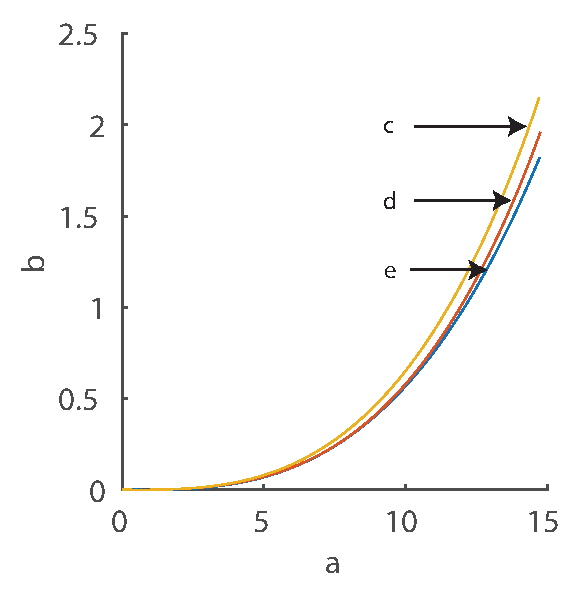
\includegraphics[width=0.45\columnwidth]{./figures/cornering_position_015_b.eps} \label{fig:corneringPosition}} \hspace{0.1cm}
      %
      \psfrag{a}[c][c]{time $t$}
      \psfrag{b}[c][c]{slip angle $\beta$}
      %
      \subfigure[Slip angle.]        
	  {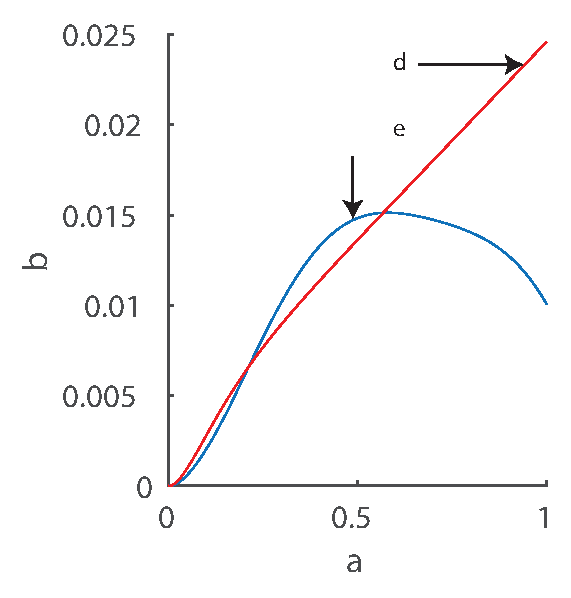
\includegraphics[width=0.45\columnwidth]{./figures/cornering_slipAngle_015_b.eps} \label{fig:corneringSlipAngle}}

      \caption{Comparing the kinematic single-track (KS) model, the single-track (ST) model and the multi-body (MB) model during cornering.}
\end{figure}

\paragraph{Overstering and understeering of the multi-body model}

During cornering, a vehicle tends to understeer when braking since typically more braking force is applied at the front brakes: Oversteering during braking would make a vehicle much less safe to drive. Oversteering can be achieved by accelerating with a rear-wheel-drive vehicle during cornering. Fig.~\ref{fig:cornerBrakeAcc_position} shows the paths of the multi-body model when using again $v_\delta = 0.15$~[rad/s] and in addition $a_\mathtt{long} = -0.7$~g for braking and $a_\mathtt{long} = 0.63$~g for acceleration. The tightest bend is realized by braking since the velocity drops and the widest bend is caused by accelerating since the velocity increases. It is evident that during braking we have understeer and during acceleration we have oversteer by observing the slip angle in Fig.~\ref{fig:cornerBrakeAcc_slipAngle}. This is also obvious from the orientation of the vehicle, where during acceleration, the vehicle turns into the corner as shown in Fig.~\ref{fig:cornerBrakeAcc_orientation}. Further, in Fig.~\ref{fig:cornerBrakeAcc_pitch} the pitch for braking shows that the vehicle is ``diving'' while the front lifts during acceleration. This plot also nicely shows the oscillation in the spring-mass-damper system since braking and acceleration is suddenly applied.

\begin{figure}[h!tb]	
    \centering	
    \footnotesize
      \psfrag{a}[c][c]{x-position $s_x$}
      \psfrag{b}[c][c]{y-position $s_y$}
      \psfrag{c}[r][c]{\shortstack{coasting}}
      \psfrag{d}[r][c]{\shortstack{braking}}
      \psfrag{e}[r][c]{\shortstack{accelerating}}
      %
      \subfigure[Path of center of gravity.] 
	  {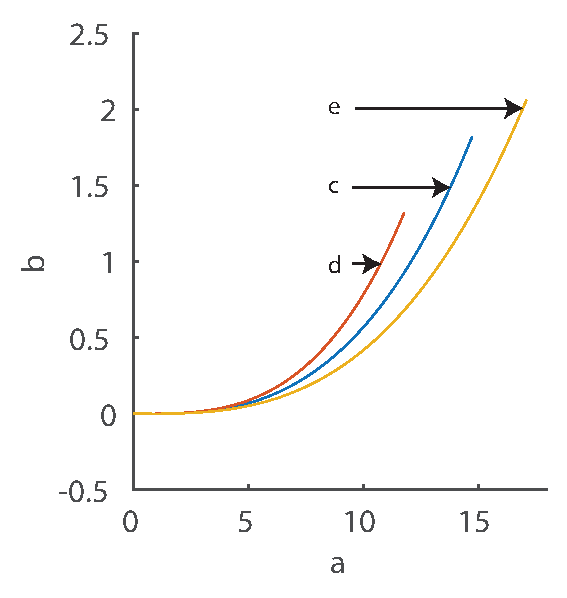
\includegraphics[width=0.45\columnwidth]{./figures/position_cornerBrakeAcc_b.eps} \label{fig:cornerBrakeAcc_position}} \hspace{0.1cm}
      %
      \psfrag{a}[c][c]{time $t$}
      \psfrag{b}[c][c]{slip angle $\beta$}
      %
      \subfigure[Slip angle.]        
	  {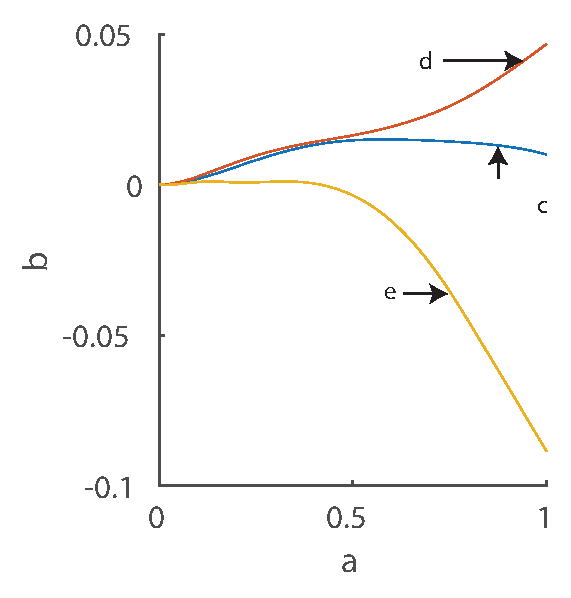
\includegraphics[width=0.45\columnwidth]{./figures/slipAngle_cornerBrakeAcc_b.eps} \label{fig:cornerBrakeAcc_slipAngle}} \\
      %
      \psfrag{a}[c][c]{time $t$}
      \psfrag{b}[c][c]{orientation $\Psi$}
      %
      \subfigure[Orientation.]        
	  {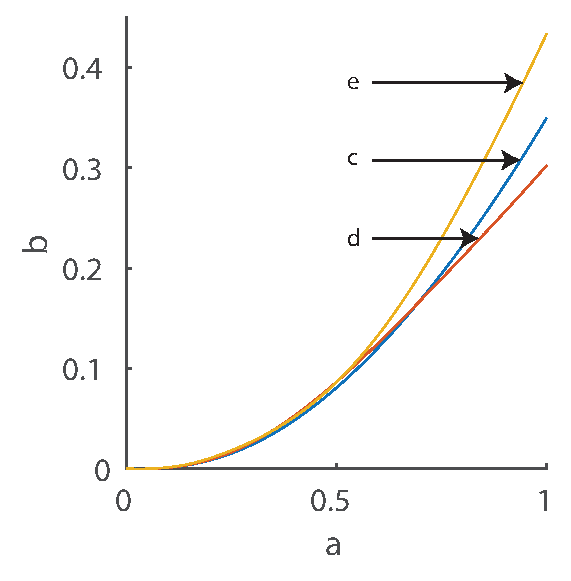
\includegraphics[width=0.45\columnwidth]{./figures/orientation_cornerBrakeAcc_b.eps} \label{fig:cornerBrakeAcc_orientation}} \hspace{0.1cm}
      %
      \psfrag{a}[c][c]{time $t$}
      \psfrag{b}[c][c]{pitch $\Theta_S$}
      %
      \subfigure[Pitch.]        
	  {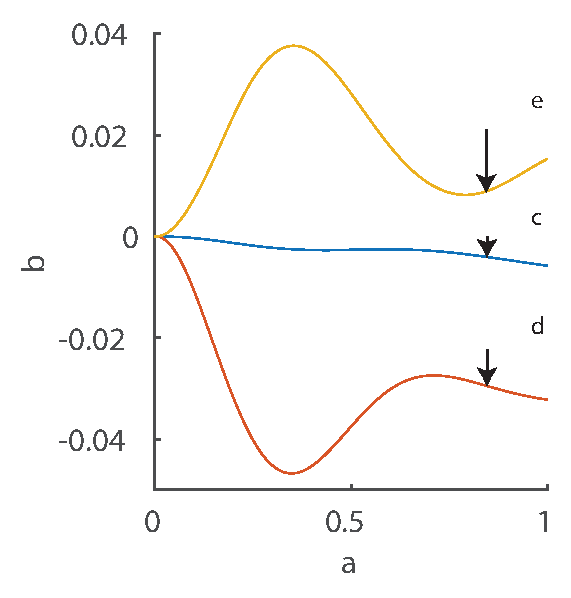
\includegraphics[width=0.45\columnwidth]{./figures/pitch_cornerBrakeAcc_b.eps} \label{fig:cornerBrakeAcc_pitch}} 

      \caption{Investigating oversteering and understeering for the multi-body model.}
\end{figure}


\section{Conclusions}

This document describes four models for motion planning of automated vehicles as part of the \textit{CommonRoad} benchmark suite: point-mass model, kinematic single-track model, single-track model, and a multi-body model. To easily exchange models, we also present how to convert parameters and initial states from the multi-body model to simpler models. The sources of all equations are carefully referenced in this work and all models are available as MATLAB and Python code. Numerical experiments provide further insight into what effects certain models can show. 


\section*{Acknowledgment}

\vspace{-0.2cm}
The author gratefully acknowledge financial support by the Free State of Bavaria.



\label{sec:bib}
\bibliographystyle{plain}
%\bibliographystyle{alpha}
%\bibliographystyle{unsrt}
%\bibliographystyle{abbrv}
\bibliography{althoff_own,althoff_other}


\end{document}

% EOF
